%% ============================================================================
%%  Language Models Meet Symbolic Reasoning:
%%  A Scoping Review of Neurosymbolic Integration at Top-Tier AI and NLP Venues
%%
%%  IEEEtran. Compile with pdfLaTeX + BibTeX (Overleaf default). Every count in
%%  the text is a \cnt{...} macro from tables/numbers.tex, regenerated by
%%  `python code/run_all.py --sources <dir>`. The full list of included studies
%%  is in supplement.tex (a separate document).
%% ============================================================================
\documentclass[conference]{IEEEtran}
\IEEEoverridecommandlockouts

\usepackage[T1]{fontenc}
\usepackage[utf8]{inputenc}
\usepackage{cite}
\usepackage{amsmath,amssymb}
\usepackage{graphicx}
\usepackage{booktabs}
\usepackage{array}
\usepackage{tabularx}
\usepackage[table]{xcolor}
\usepackage{listings}
\usepackage{pifont}
\usepackage{tikz}
\usetikzlibrary{positioning,arrows.meta,fit,calc,shapes.geometric,backgrounds}
\usepackage{pgfplots}
\pgfplotsset{compat=1.18}
\usepackage{pgfplotstable}
\usepackage{url}
\usepackage[hidelinks]{hyperref}

\definecolor{nsblue}{RGB}{37,99,235}
\definecolor{nsgrey}{RGB}{120,120,120}
\definecolor{nslight}{RGB}{226,232,240}
\definecolor{A1c}{RGB}{37,99,235}
\definecolor{A2c}{RGB}{14,165,233}
\definecolor{A3c}{RGB}{16,185,129}
\definecolor{A4c}{RGB}{245,158,11}
\definecolor{A5c}{RGB}{239,68,68}
\definecolor{A6c}{RGB}{139,92,246}
\definecolor{A7c}{RGB}{100,116,139}

% Auto-generated by code/s07_build_latex.py -- do not edit by hand.
\makeatletter
\expandafter\def\csname cnt@identified\endcsname{391}
\expandafter\def\csname cnt@withpdf\endcsname{368}
\expandafter\def\csname cnt@duplicates\endcsname{4}
\expandafter\def\csname cnt@screened\endcsname{387}
\expandafter\def\csname cnt@exclscreen\endcsname{290}
\expandafter\def\csname cnt@filterhits\endcsname{93}
\expandafter\def\csname cnt@titleadds\endcsname{4}
\expandafter\def\csname cnt@abstracts\endcsname{367}
\expandafter\def\csname cnt@titlereviewed\endcsname{93}
\expandafter\def\csname cnt@notflagged\endcsname{294}
\expandafter\def\csname cnt@assessed\endcsname{97}
\expandafter\def\csname cnt@exclelig\endcsname{24}
\expandafter\def\csname cnt@included\endcsname{73}
\expandafter\def\csname cnt@includedpct\endcsname{19}
\expandafter\def\csname cnt@pubabstract\endcsname{4}
\expandafter\def\csname cnt@fulltext\endcsname{69}
\expandafter\def\csname cnt@artifact\endcsname{37}
\expandafter\def\csname cnt@artifactpct\endcsname{54}
\expandafter\def\csname cnt@threshold\endcsname{3}
\expandafter\def\csname cnt@spotn\endcsname{20}
\expandafter\def\csname cnt@spotok\endcsname{19}
\expandafter\def\csname cnt@nolmfamily\endcsname{12}
\expandafter\def\csname cnt@early\endcsname{8}
\expandafter\def\csname cnt@late\endcsname{65}
\expandafter\def\csname cnt@spotonen\endcsname{20}
\expandafter\def\csname cnt@spotoneok\endcsname{15}
\expandafter\def\csname cnt@replayflagged\endcsname{387}
\expandafter\def\csname cnt@replaycore\endcsname{149}
\expandafter\def\csname cnt@replayadjacent\endcsname{238}
\expandafter\def\csname cnt@replaymissed\endcsname{4}
\expandafter\def\csname cnt@replaypct\endcsname{99.0}
\expandafter\def\csname cnt@studieswithlmfamily\endcsname{57}
\expandafter\def\csname cnt@studieswithbenchmark\endcsname{32}
\expandafter\def\csname cnt@studieswithengine\endcsname{27}
\expandafter\def\csname cnt@proprietaryany\endcsname{45}
\expandafter\def\csname cnt@openany\endcsname{46}
\expandafter\def\csname cnt@both\endcsname{34}
\expandafter\def\csname cnt@openonly\endcsname{12}
\expandafter\def\csname cnt@proprietaryonly\endcsname{11}
\expandafter\def\csname cnt@indGPT4\endcsname{32}
\expandafter\def\csname cnt@indLlama\endcsname{21}
\expandafter\def\csname cnt@indDeepSeek\endcsname{21}
\expandafter\def\csname cnt@indGPT35\endcsname{18}
\expandafter\def\csname cnt@indQwen\endcsname{16}
\expandafter\def\csname cnt@indClaude\endcsname{7}
\expandafter\def\csname cnt@indGemini\endcsname{6}
\expandafter\def\csname cnt@indLLaVA\endcsname{5}
\expandafter\def\csname cnt@indGPT3\endcsname{5}
\expandafter\def\csname cnt@indT5\endcsname{4}
\expandafter\def\csname cnt@indMistral\endcsname{4}
\expandafter\def\csname cnt@indInternLM\endcsname{3}
\expandafter\def\csname cnt@indBERT\endcsname{2}
\expandafter\def\csname cnt@indChinchilla\endcsname{1}
\expandafter\def\csname cnt@indLean\endcsname{13}
\expandafter\def\csname cnt@indZ3\endcsname{9}
\expandafter\def\csname cnt@indIsabelle\endcsname{5}
\expandafter\def\csname cnt@indPDDL\endcsname{3}
\expandafter\def\csname cnt@indProlog\endcsname{3}
\expandafter\def\csname cnt@indASP\endcsname{3}
\expandafter\def\csname cnt@indCoq\endcsname{2}
\expandafter\def\csname cnt@indSymPy\endcsname{2}
\expandafter\def\csname cnt@indProver9\endcsname{2}
\expandafter\def\csname cnt@indminiF2F\endcsname{7}
\expandafter\def\csname cnt@indFOLIO\endcsname{5}
\expandafter\def\csname cnt@indProofNet\endcsname{4}
\expandafter\def\csname cnt@indARC\endcsname{4}
\expandafter\def\csname cnt@indSRBench\endcsname{4}
\expandafter\def\csname cnt@indALFWorld\endcsname{4}
\expandafter\def\csname cnt@indProofWriter\endcsname{4}
\expandafter\def\csname cnt@indCLEVR\endcsname{3}
\expandafter\def\csname cnt@indPrOntoQA\endcsname{3}
\expandafter\def\csname cnt@indMATH\endcsname{2}
\expandafter\def\csname cnt@indVirtualHome\endcsname{2}
\expandafter\def\csname cnt@indGSM8K\endcsname{1}
\expandafter\def\csname cnt@indSpider\endcsname{1}
\expandafter\def\csname cnt@indGQA\endcsname{1}
\expandafter\def\csname cnt@E1\endcsname{3}
\expandafter\def\csname cnt@E2\endcsname{8}
\expandafter\def\csname cnt@E3\endcsname{8}
\expandafter\def\csname cnt@E4\endcsname{3}
\expandafter\def\csname cnt@E5\endcsname{2}
\expandafter\def\csname cnt@D7\endcsname{6}
\expandafter\def\csname cnt@D5\endcsname{11}
\expandafter\def\csname cnt@D3\endcsname{10}
\expandafter\def\csname cnt@D1\endcsname{14}
\expandafter\def\csname cnt@D2\endcsname{16}
\expandafter\def\csname cnt@D4\endcsname{4}
\expandafter\def\csname cnt@D6\endcsname{12}
\expandafter\def\csname cnt@A3\endcsname{18}
\expandafter\def\csname cnt@A7\endcsname{5}
\expandafter\def\csname cnt@A2\endcsname{13}
\expandafter\def\csname cnt@A6\endcsname{9}
\expandafter\def\csname cnt@A1\endcsname{10}
\expandafter\def\csname cnt@A5\endcsname{4}
\expandafter\def\csname cnt@A4\endcsname{14}
\expandafter\def\csname cnt@F7\endcsname{9}
\expandafter\def\csname cnt@F3\endcsname{13}
\expandafter\def\csname cnt@F2\endcsname{14}
\expandafter\def\csname cnt@F1\endcsname{22}
\expandafter\def\csname cnt@F4\endcsname{4}
\expandafter\def\csname cnt@F5\endcsname{6}
\expandafter\def\csname cnt@F6\endcsname{5}
\expandafter\def\csname cnt@ICML\endcsname{19}
\expandafter\def\csname cnt@NeurIPS\endcsname{14}
\expandafter\def\csname cnt@AAAI\endcsname{16}
\expandafter\def\csname cnt@IJCAI\endcsname{4}
\expandafter\def\csname cnt@TMLR\endcsname{4}
\expandafter\def\csname cnt@ICLR\endcsname{15}
\expandafter\def\csname cnt@TPAMI\endcsname{1}
\expandafter\def\csname cnt@y2020\endcsname{1}
\expandafter\def\csname cnt@s2020\endcsname{39}
\expandafter\def\csname cnt@share2020\endcsname{3}
\expandafter\def\csname cnt@y2021\endcsname{3}
\expandafter\def\csname cnt@s2021\endcsname{36}
\expandafter\def\csname cnt@share2021\endcsname{8}
\expandafter\def\csname cnt@y2022\endcsname{2}
\expandafter\def\csname cnt@s2022\endcsname{47}
\expandafter\def\csname cnt@share2022\endcsname{4}
\expandafter\def\csname cnt@y2023\endcsname{2}
\expandafter\def\csname cnt@s2023\endcsname{63}
\expandafter\def\csname cnt@share2023\endcsname{3}
\expandafter\def\csname cnt@y2024\endcsname{13}
\expandafter\def\csname cnt@s2024\endcsname{59}
\expandafter\def\csname cnt@share2024\endcsname{22}
\expandafter\def\csname cnt@y2025\endcsname{29}
\expandafter\def\csname cnt@s2025\endcsname{96}
\expandafter\def\csname cnt@share2025\endcsname{30}
\expandafter\def\csname cnt@y2026\endcsname{23}
\expandafter\def\csname cnt@s2026\endcsname{47}
\expandafter\def\csname cnt@share2026\endcsname{49}
\expandafter\def\csname cnt@D7A3\endcsname{2}
\expandafter\def\csname cnt@D5A7\endcsname{1}
\expandafter\def\csname cnt@D3A3\endcsname{6}
\expandafter\def\csname cnt@D1A2\endcsname{6}
\expandafter\def\csname cnt@D3A2\endcsname{2}
\expandafter\def\csname cnt@D2A6\endcsname{4}
\expandafter\def\csname cnt@D1A3\endcsname{4}
\expandafter\def\csname cnt@D1A1\endcsname{1}
\expandafter\def\csname cnt@D4A2\endcsname{2}
\expandafter\def\csname cnt@D6A5\endcsname{1}
\expandafter\def\csname cnt@D1A6\endcsname{2}
\expandafter\def\csname cnt@D5A4\endcsname{5}
\expandafter\def\csname cnt@D2A3\endcsname{3}
\expandafter\def\csname cnt@D7A4\endcsname{2}
\expandafter\def\csname cnt@D6A6\endcsname{3}
\expandafter\def\csname cnt@D7A5\endcsname{2}
\expandafter\def\csname cnt@D4A4\endcsname{1}
\expandafter\def\csname cnt@D5A2\endcsname{2}
\expandafter\def\csname cnt@D3A4\endcsname{2}
\expandafter\def\csname cnt@D5A5\endcsname{1}
\expandafter\def\csname cnt@D5A3\endcsname{2}
\expandafter\def\csname cnt@D6A4\endcsname{3}
\expandafter\def\csname cnt@D6A1\endcsname{1}
\expandafter\def\csname cnt@D6A7\endcsname{4}
\expandafter\def\csname cnt@D2A2\endcsname{1}
\expandafter\def\csname cnt@D2A1\endcsname{8}
\expandafter\def\csname cnt@D1A4\endcsname{1}
\expandafter\def\csname cnt@D4A3\endcsname{1}
\expandafter\def\csname cnt@themeabductivelearning\endcsname{15}
\expandafter\def\csname cnt@themeincabductivelearning\endcsname{1}
\expandafter\def\csname cnt@themeprobabilisticlogic\endcsname{26}
\expandafter\def\csname cnt@themeincprobabilisticlogic\endcsname{1}
\expandafter\def\csname cnt@themedifferentiableorfuzzylogic\endcsname{10}
\expandafter\def\csname cnt@themeincdifferentiableorfuzzylogic\endcsname{1}
\expandafter\def\csname cnt@themereasoningshortcuts\endcsname{8}
\expandafter\def\csname cnt@themeincreasoningshortcuts\endcsname{0}
\expandafter\def\csname cnt@themesymbolicregression\endcsname{44}
\expandafter\def\csname cnt@themeincsymbolicregression\endcsname{4}
\expandafter\def\csname cnt@themeinductivelogicprogramming\endcsname{31}
\expandafter\def\csname cnt@themeincinductivelogicprogramming\endcsname{0}
\expandafter\def\csname cnt@kappa\endcsname{0.77}
\expandafter\def\csname cnt@rawagree\endcsname{91.8}
\expandafter\def\csname cnt@kappan\endcsname{97}
\expandafter\def\csname cnt@ndisagree\endcsname{8}
\expandafter\def\csname cnt@secondincluded\endcsname{72}
\expandafter\def\csname cnt@firstincluded\endcsname{76}
\expandafter\def\csname cnt@resolvedsecond\endcsname{3}
\expandafter\def\csname cnt@resolvedfirst\endcsname{4}
\expandafter\def\csname cnt@resolvedcode\endcsname{1}
\expandafter\def\csname cnt@chisq\endcsname{84.4}
\expandafter\def\csname cnt@cramerv\endcsname{0.44}
\expandafter\def\csname cnt@permp\endcsname{0.0001}
\expandafter\def\csname cnt@nperm\endcsname{10{,}000}
\newcommand{\cnt}[1]{\@ifundefined{cnt@#1}{\textbf{??#1??}}{\csname cnt@#1\endcsname}}
\makeatother
\makeatletter
\expandafter\def\csname cnt@earlyA1\endcsname{0}
\expandafter\def\csname cnt@earlyA2\endcsname{0}
\expandafter\def\csname cnt@earlyA3\endcsname{5}
\expandafter\def\csname cnt@earlyA4\endcsname{2}
\expandafter\def\csname cnt@earlyA5\endcsname{0}
\expandafter\def\csname cnt@earlyA6\endcsname{1}
\expandafter\def\csname cnt@earlyA7\endcsname{0}
\expandafter\def\csname cnt@earlyAoneAtwo\endcsname{0}
\expandafter\def\csname cnt@earlytotal\endcsname{8}
\expandafter\def\csname cnt@y2024A1\endcsname{1}
\expandafter\def\csname cnt@y2024A2\endcsname{2}
\expandafter\def\csname cnt@y2024A3\endcsname{4}
\expandafter\def\csname cnt@y2024A4\endcsname{3}
\expandafter\def\csname cnt@y2024A5\endcsname{1}
\expandafter\def\csname cnt@y2024A6\endcsname{0}
\expandafter\def\csname cnt@y2024A7\endcsname{2}
\expandafter\def\csname cnt@y2024AoneAtwo\endcsname{3}
\expandafter\def\csname cnt@y2024total\endcsname{13}
\expandafter\def\csname cnt@y2025A1\endcsname{4}
\expandafter\def\csname cnt@y2025A2\endcsname{6}
\expandafter\def\csname cnt@y2025A3\endcsname{7}
\expandafter\def\csname cnt@y2025A4\endcsname{5}
\expandafter\def\csname cnt@y2025A5\endcsname{2}
\expandafter\def\csname cnt@y2025A6\endcsname{5}
\expandafter\def\csname cnt@y2025A7\endcsname{0}
\expandafter\def\csname cnt@y2025AoneAtwo\endcsname{10}
\expandafter\def\csname cnt@y2025total\endcsname{29}
\expandafter\def\csname cnt@y2026A1\endcsname{5}
\expandafter\def\csname cnt@y2026A2\endcsname{5}
\expandafter\def\csname cnt@y2026A3\endcsname{2}
\expandafter\def\csname cnt@y2026A4\endcsname{4}
\expandafter\def\csname cnt@y2026A5\endcsname{1}
\expandafter\def\csname cnt@y2026A6\endcsname{3}
\expandafter\def\csname cnt@y2026A7\endcsname{3}
\expandafter\def\csname cnt@y2026AoneAtwo\endcsname{10}
\expandafter\def\csname cnt@y2026total\endcsname{23}
\makeatother
\makeatletter
\expandafter\def\csname cnt@artA1\endcsname{90}
\expandafter\def\csname cnt@artnA1\endcsname{10}
\expandafter\def\csname cnt@artyA1\endcsname{9}
\expandafter\def\csname cnt@artA2\endcsname{54}
\expandafter\def\csname cnt@artnA2\endcsname{13}
\expandafter\def\csname cnt@artyA2\endcsname{7}
\expandafter\def\csname cnt@artA3\endcsname{44}
\expandafter\def\csname cnt@artnA3\endcsname{16}
\expandafter\def\csname cnt@artyA3\endcsname{7}
\expandafter\def\csname cnt@artA4\endcsname{43}
\expandafter\def\csname cnt@artnA4\endcsname{14}
\expandafter\def\csname cnt@artyA4\endcsname{6}
\expandafter\def\csname cnt@artA5\endcsname{50}
\expandafter\def\csname cnt@artnA5\endcsname{4}
\expandafter\def\csname cnt@artyA5\endcsname{2}
\expandafter\def\csname cnt@artA6\endcsname{67}
\expandafter\def\csname cnt@artnA6\endcsname{9}
\expandafter\def\csname cnt@artyA6\endcsname{6}
\expandafter\def\csname cnt@artA7\endcsname{0}
\expandafter\def\csname cnt@artnA7\endcsname{3}
\expandafter\def\csname cnt@artyA7\endcsname{0}
\makeatother
   % \cnt{...} and \ifhumancheck
\newcommand{\pendingbox}[1]{\fbox{\parbox{0.95\linewidth}{\raggedright\color{red}\footnotesize\textbf{AUTHOR ACTION REQUIRED:} #1}}}
\newcommand{\RQ}[1]{\textbf{RQ#1}}

\lstset{basicstyle=\ttfamily\scriptsize, breaklines=true, breakatwhitespace=false, columns=fullflexible,
        frame=single, rulecolor=\color{nsgrey}, keepspaces=true, backgroundcolor=\color{nslight!40}}

\begin{document}

\title{Language Models Meet Symbolic Reasoning:\\
A Scoping Review of Neurosymbolic Integration at Top-Tier AI and NLP Venues (2020--2026)}

\author{\IEEEauthorblockN{Jatin Thakur}
\IEEEauthorblockA{\textit{Jaypee University of Information Technology (JUIT)}\\
Waknaghat, Solan, Himachal Pradesh, India\\
jatinthakur3333@gmail.com}}

\maketitle

\begin{abstract}
Large language models (LLMs) can write code, propose proof steps and translate problems into formal languages, but their outputs carry no guarantee of correctness; symbolic systems give exact verdicts but need formal input. We report a scoping review, following PRISMA-ScR, of how language models---from pretrained sequence models to LLMs---and explicit symbolic components are integrated in work published at ten top-tier AI and NLP venues from 2020 to 2026. We searched the titles and abstracts of \cnt{sourceb} accepted papers, combined the hits with a curated neurosymbolic corpus, snowballed from included studies and audited a stratified sample of non-retrieved records, which yields an estimated search recall of \cnt{recallpoint} (95\% interval \cnt{recalllo}--\cnt{recallhi}). Screening and data charting were carried out by independent LLM-based reviewers with adjudication under a published protocol (screening $\kappa=\cnt{kappaunion}$; coding $\kappa=\cnt{kappaarch}$--\cnt{kappaform} per axis), \ifhumancheck and a human check of a 30\% sample gave $\kappa=\cnt{humscrkappa}$ against the final screening decisions\else and we release a blinded 30\% sample for human verification\fi. We include \cnt{included} studies. Normalised by accepted papers, such work grew from \cnt{pfive2020} to \cnt{pfive2025} studies per 1{,}000 papers between 2020 and 2025, while only \cnt{nesytitlepct}\% of the studies call themselves neurosymbolic in their title. We identify seven integration architectures; architecture is moderately associated with task domain (bias-corrected Cram\'er's $V=\cnt{Vcall}$), and designs in which a symbolic checker gives verdicts on model outputs rose from \cnt{earlyAtwo}\% of studies in 2020--2022 to \cnt{ysixAtwo}\% in 2026. Only \cnt{faithyes} of \cnt{faithn} studies whose model writes formal statements report formalisation faithfulness in the abstract, \cnt{benchsinglepct}\% of named benchmarks appear in a single study, and an estimated \cnt{artrandrate}\% (95\% CI \cnt{artrandlo}--\cnt{artrandhi}) of studies release code or data. We release all decisions, prompts and a pipeline that regenerates every number in the paper.
\end{abstract}

\begin{IEEEkeywords}
neurosymbolic AI, large language models, symbolic reasoning, theorem proving, program synthesis, scoping review, PRISMA-ScR
\end{IEEEkeywords}

\section{Introduction}
\label{sec:intro}

Neurosymbolic AI pursues systems that learn from data like neural networks and reason with explicit structure like symbolic programs~\cite{garcez2023neurosymbolic,kautz2022third,deraedt2020statistical}. For most of the last decade its flagship techniques were differentiable or probabilistic logics trained end to end with perception networks~\cite{manhaeve2018deepproblog,yang2020neurasp,huang2021scallop}. Pretrained language models changed the question. A model can now write the formal specification~\cite{wu2022autoformalization,olausson2023linc}, propose the next proof tactic~\cite{polu2020generative,yang2023leandojo} or generate a program~\cite{gao2023pal,cheng2023binding}, and an exact engine can then check, execute or solve what it wrote. The central design decision has moved from \emph{how to make logic differentiable} to \emph{how to divide labour between a pretrained model and an exact engine}.

The literature on this division of labour is large and fast-moving but reported piecemeal. Recent surveys organise it narratively~\cite{yang2025neuro,cheng2025empowering,rani2025advancing}, and the most recent systematic review of neurosymbolic AI~\cite{colelough2025neurosymbolic} does not single out language models. Basic questions therefore lack evidence-based answers. Which integration patterns exist and how common are they? Does the pattern depend on the task? Which models, engines and benchmarks does the community use, and how often are results reproducible? Has the field shifted over time, or is the apparent growth an artefact of terminology?

This paper answers these questions with a \emph{scoping review}~\cite{arksey2005scoping} reported according to PRISMA-ScR~\cite{tricco2018prisma}. A scoping review maps the extent and nature of a body of evidence rather than pooling effect sizes, which matches our aim. We define the population as work published at ten top-tier venues---AAAI, IJCAI, ICLR, ICML, NeurIPS, ACL, EMNLP, NAACL, TMLR and IEEE TPAMI---between 2020 and 2026, because these venues set the methodological agenda of both the machine-learning and the NLP communities and fix a quality floor. We include every study in which a language model and an explicit symbolic component \emph{interact}.

\subsection{Research questions}
\begin{itemize}
  \item[\RQ{1}] \emph{Architectures.} What architectures connect language models to symbolic components, how often is each used, and what kind of check does the symbolic side provide?
  \item[\RQ{2}] \emph{Tasks and formalisms.} Which task domains and formalisms do the architectures serve, and is architecture associated with domain?
  \item[\RQ{3}] \emph{Evaluation and reproducibility.} Which models, engines and benchmarks are used, what do studies report about the faithfulness of formalisation, and how often are artifacts released?
  \item[\RQ{4}] \emph{Trends.} How has the area changed from 2020 to 2026 once growth in the venues themselves is accounted for?
\end{itemize}

\subsection{Contributions}
\begin{enumerate}
  \item \textbf{A recall-audited evidence base.} An abstract-level search of \cnt{sourceb} accepted papers, combined with a curated corpus, backward snowballing and a stratified audit of non-retrieved records, yields \cnt{included} studies and a quantified estimate of search recall (Sections~\ref{sec:method}--\ref{sec:selection}).
  \item \textbf{A transparent, double-coded taxonomy.} Seven integration architectures assigned by an ordered decision tree, a check-strength attribute, eight domains and seven formalisms, each coded twice independently with per-axis agreement (Sections~\ref{sec:taxonomy}--\ref{sec:domains}).
  \item \textbf{Evidence on evaluation practice.} Open-vocabulary extraction of models, engines and benchmarks; coded reporting of formalisation faithfulness; a web-verified estimate of artifact release; and a results-level view of the most shared benchmark (Section~\ref{sec:evaluation}).
  \item \textbf{Venue-normalised trends} with a terminology control (Section~\ref{sec:trends}) and a research agenda grounded in the coded evidence (Section~\ref{sec:challenges}).
  \item \textbf{A replication package.} Every screening and coding decision, every prompt given to an LLM reviewer and a dependency-free pipeline that regenerates every number in this paper from public sources at fixed commits.
\end{enumerate}

We are explicit about one methodological choice throughout: screening and coding were performed by LLM-based reviewers under a fixed protocol, with independent double assessment and adjudication. Section~\ref{sec:method-ai} describes the arrangement and Section~\ref{sec:validity} its limits.

Section~\ref{sec:background} positions the study. Section~\ref{sec:method} describes the protocol. Sections~\ref{sec:selection}--\ref{sec:trends} report results for \RQ{1}--\RQ{4}. Section~\ref{sec:challenges} sets out open challenges, Section~\ref{sec:validity} threats to validity, and Section~\ref{sec:conclusion} concludes.

\section{Background and Related Surveys}
\label{sec:background}

\subsection{Neurosymbolic integration before language models}
Neurosymbolic AI combines sub-symbolic learning with symbolic knowledge and inference~\cite{garcez2023neurosymbolic}. Kautz~\cite{kautz2022third} distinguishes integration types ranging from \emph{Neuro|Symbolic} pipelines, in which a neural front end feeds a symbolic reasoner, to \emph{Neuro$_\text{Symbolic}$} systems in which rules act as a training signal. De Raedt et al.~\cite{deraedt2020statistical} relate the field to statistical relational AI and classify systems by the type of logic, the treatment of symbols and the degree of integration. Representative systems of this period are probabilistic logic programs with neural predicates~\cite{manhaeve2018deepproblog,yang2020neurasp,huang2021scallop}, whose exact inference is provably hard~\cite{maene2024hardness} and motivates approximations~\cite{vankrieken2023nesi}. A recurring concern is \emph{reasoning shortcuts}: models that satisfy symbolic constraints for the wrong reasons~\cite{marconato2023neuro,yang2024analysis}.

\subsection{Why language models change the design space}
Pretrained language models bring three capabilities that earlier neurosymbolic systems lacked. They map unstructured problems to formal languages without task-specific training, enabling pipelines in which the model formalises and an engine solves~\cite{olausson2023linc,ye2023satlm,pan2023logiclm}. They generate long structured artifacts---programs, proofs, plans---that a symbolic system can execute or check, enabling generate-and-check loops~\cite{polu2020generative,jiang2023draft}. And they carry broad world knowledge, so symbolic components can be grounded in open-vocabulary concepts rather than a fixed predicate set~\cite{gupta2023visprog,suris2023vipergpt}. Each capability changes where the symbolic component sits and what it is trusted to do, which is what our architecture axis records.

\subsection{Related surveys and the gap addressed here}
Table~\ref{tab:related} compares this review with the closest secondary studies. Surveys that focus on language models and symbolic reasoning~\cite{yang2025neuro,cheng2025empowering,rani2025advancing} are narrative: they report neither a search protocol nor a study count, so their coverage cannot be audited. Yang et al.~\cite{yang2025neuro} organise methods into Symbolic$\rightarrow$LLM, LLM$\rightarrow$Symbolic and LLM+Symbolic perspectives; our architectures refine these (Section~\ref{sec:taxonomy-relations}). Systematic reviews of neurosymbolic AI exist~\cite{colelough2025neurosymbolic,delvecchio2025neuro}, but neither isolates the integration of language models, and broad surveys of neurosymbolic computing~\cite{wang2025data,lamb2020graph,deraedt2020statistical} predate or do not centre on the language-model era.

Our review also uses LLMs as reviewers. Evaluations of GPT-4 for screening and data extraction report performance that varies with task and domain and recommend human oversight~\cite{khraisha2024can}. We therefore treat LLM-based screening as a design choice that must be disclosed, measured with independent double assessment, and checked by a human sample (Section~\ref{sec:method-ai}).

\begin{table*}[t]
\centering
\caption{Positioning against related secondary studies. ``Protocol'' means the study reports its sources, eligibility criteria and study counts. LM = language model.}
\label{tab:related}
\footnotesize
\begin{tabularx}{\textwidth}{@{}l l c c X@{}}
\toprule
Study & Venue & Protocol & LM focus & Scope and organising principle \\
\midrule
De Raedt et al.~\cite{deraedt2020statistical} & IJCAI 2020 & -- & -- & Parallels between statistical relational and neurosymbolic AI; dimensions such as logic type and degree of integration \\
Lamb et al.~\cite{lamb2020graph} & IJCAI 2020 & -- & -- & Graph neural networks as a neural-symbolic computing substrate \\
Wang et al.~\cite{wang2025data} & TPAMI 2025 & -- & -- & Narrative survey of neuro-symbolic computing; organised by integration type, knowledge representation, knowledge embedding and functionality (read from the arXiv version) \\
Delvecchio et al.~\cite{delvecchio2025neuro} & IJCAI 2025 & \checkmark & -- & Task-directed survey of neurosymbolic systems 2017--2024, collected via the DBLP SPARQL endpoint from leading venues \\
Colelough and Regli~\cite{colelough2025neurosymbolic} & arXiv 2025 & \checkmark & -- & PRISMA review: 1{,}428 screened, 167 included (2020--2024); categories such as learning and inference, knowledge representation, explainability \\
Cheng et al.~\cite{cheng2025empowering} & IJCAI 2025 & -- & \checkmark & Logical reasoning in LLMs (narrative) \\
Yang et al.~\cite{yang2025neuro} & IJCAI 2025 & -- & \checkmark & Neurosymbolic methods for LLM reasoning: Symbolic$\rightarrow$LLM, LLM$\rightarrow$Symbolic, LLM+Symbolic \\
Rani et al.~\cite{rani2025advancing} & arXiv 2025 & -- & \checkmark & Symbolic integration in LLMs: lifecycle stage, coupling, architecture, application \\
\midrule
\textbf{This review} & -- & \checkmark & \checkmark & PRISMA-ScR; \cnt{sourceb} abstracts searched + curated corpus + snowballing; recall audit; \cnt{included} studies (2020--2026); double-coded architecture, check strength, domain and formalism; executable replication package \\
\bottomrule
\end{tabularx}
\end{table*}

\section{Review Methodology}
\label{sec:method}

\subsection{Design and reporting standard}
We conducted a scoping review in the sense of Arksey and O'Malley~\cite{arksey2005scoping}: the aim is to map the extent, range and nature of the evidence, not to estimate effects. Reporting follows PRISMA-ScR~\cite{tricco2018prisma}; Appendix~\ref{app:prisma} maps every checklist item to its location. Planning and conduct also follow the systematic-mapping guidance of software engineering~\cite{petersen2008systematic,kitchenham2007guidelines}. The protocol (version 2, released with the data) fixes the eligibility rules, the screening and adjudication procedure and the coding scheme. It was not registered in advance. It replaces a pilot version that searched only the curated corpus; Section~\ref{sec:method-changes} lists the differences. Figure~\ref{fig:pipeline} summarises the workflow.

% Review workflow (v2): sources, query, two LLM screeners, adjudication, snowballing,
% recall audit, double coding, analyses. Orange = versioned decision files.
\begin{figure*}[t]
\centering
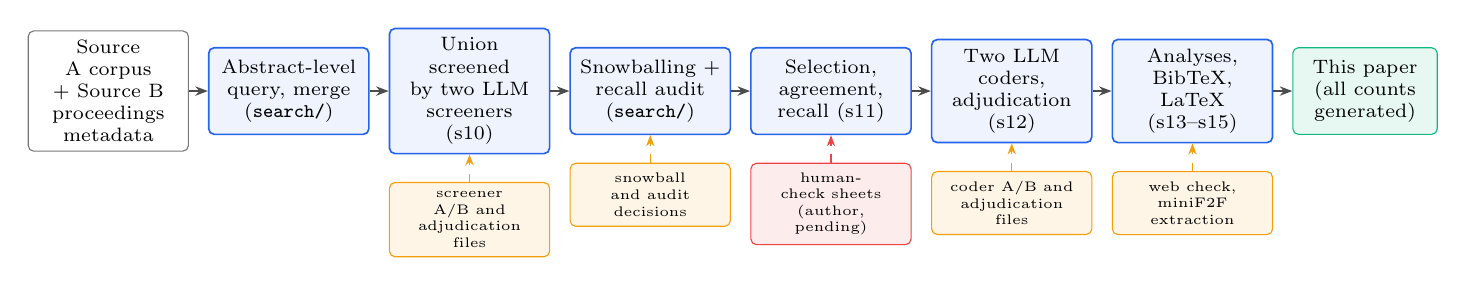
\begin{tikzpicture}[
  node distance=3.5mm and 2.4mm,
  font=\scriptsize,
  stepbox/.style={draw=nsblue, fill=nsblue!8, rounded corners=2pt, align=center, minimum height=11mm, text width=18mm, line width=0.6pt},
  ppsrc/.style={draw=nsgrey, fill=white, rounded corners=2pt, align=center, minimum height=11mm, text width=18mm},
  ppman/.style={draw=A4c, fill=A4c!10, rounded corners=2pt, align=center, minimum height=8mm, text width=18mm, font=\tiny},
  ppout/.style={draw=A3c, fill=A3c!10, rounded corners=2pt, align=center, minimum height=11mm, text width=16mm},
  arr/.style={-{Stealth[length=1.6mm]}, line width=0.5pt, draw=black!70},
  marr/.style={-{Stealth[length=1.4mm]}, line width=0.5pt, draw=A4c, dashed}]
\node[ppsrc] (srcs) {Source A corpus\\+ Source B\\proceedings\\metadata};
\node[stepbox, right=of srcs] (q) {Abstract-level\\query, merge\\(\texttt{search/})};
\node[stepbox, right=of q] (s10) {Union screened\\by two LLM\\screeners (s10)};
\node[stepbox, right=of s10] (sn) {Snowballing +\\recall audit\\(\texttt{search/})};
\node[stepbox, right=of sn] (s11) {Selection,\\agreement,\\recall (s11)};
\node[stepbox, right=of s11] (s12) {Two LLM coders,\\adjudication\\(s12)};
\node[stepbox, right=of s12] (s13) {Analyses,\\BibTeX, LaTeX\\(s13--s15)};
\node[ppout, right=of s13] (paper) {This paper\\(all counts\\generated)};
\node[ppman, below=of s10] (m1) {screener A/B and\\adjudication files};
\node[ppman, below=of sn] (m2) {snowball and audit\\decisions};
\node[ppman, below=of s12] (m3) {coder A/B and\\adjudication files};
\node[ppman, below=of s13] (m4) {web check, miniF2F\\extraction};
\node[ppman, below=of s11, fill=A5c!10, draw=A5c] (h) {human-check sheets\\(author, pending)};
\foreach \a/\b in {srcs/q,q/s10,s10/sn,sn/s11,s11/s12,s12/s13,s13/paper} \draw[arr] (\a) -- (\b);
\foreach \a/\b in {m1/s10,m2/sn,m3/s12,m4/s13} \draw[marr] (\a) -- (\b);
\draw[marr, draw=A5c] (h) -- (s11);
\end{tikzpicture}
\caption{Review workflow. Blue boxes are scripts in the replication package; orange boxes are versioned decision files written by the independent LLM screeners, coders, adjudicators and web checkers (all prompts released), which the scripts read but never modify. The red box is the human-verification sample (Section~\ref{sec:method-human}). Consistency checks stop the pipeline if a record lacks a decision or an adjudication is missing or superfluous.}
\label{fig:pipeline}
\end{figure*}


\subsection{Eligibility criteria}
\label{sec:method-eligibility}
A study is included when all of I1--I4 hold (Table~\ref{tab:criteria}). I1 restricts the population to archival research papers at ten venues: AAAI (technical track), IJCAI (main and special tracks), ICLR, ICML, NeurIPS (main and Datasets \& Benchmarks), ACL, EMNLP and NAACL (main conference), TMLR and IEEE TPAMI, 2020--2026. I2 and I3 together require that a language model and an explicit symbolic component \emph{interact}. Six rules make this boundary operational.
\begin{itemize}
  \item \emph{R1 (language model).} A neural sequence model trained or pretrained on natural-language, mathematical-text or source-code corpora, at any scale from LSTM language models to LLMs, or a vision-language model built on one. A sequence model trained only on task-generated symbolic data (for example, a transformer trained from scratch to emit expression trees) does not qualify.
  \item \emph{R2 (interaction).} The output of one component is the input, constraint, verdict or training signal of the other. Portfolios that merely choose between a model and a solver do not qualify. Evaluation studies qualify when a symbolic system generates the problems or certifies the answers the model is scored against.
  \item \emph{R3 (symbolic component).} A system that represents knowledge or computation in an explicit formal language and manipulates it by rule-governed procedures: solvers, provers and proof assistants, logic and answer-set programs, planners, model checkers, interpreters executing model-written programs, computer algebra, symbolic search, and grammars, automata or static analyses that constrain or check the model. Natural-language reasoning chains, text retrieval stores and neural modules without a formal representation do not qualify.
  \item \emph{R4 (program and query generation).} For code generation evaluated by tests, text-to-SQL and knowledge-base question answering by query generation, executing the generated program does not by itself satisfy I3; an additional symbolic component (verifier, type or dataflow analysis, grammar-based checker, symbolic search) is required. When a program is the \emph{vehicle} for another task---mathematics, tables, puzzles, planning, robot control, visual reasoning---I3 is satisfied.
  \item \emph{R5 (knowledge graphs).} A knowledge graph counts only when the method performs logical inference over it; retrieving triples into a prompt does not.
  \item \emph{R6 (tool use).} Generic multi-tool frameworks do not satisfy I3 unless a specific formal engine under R3 is the object of the integration.
\end{itemize}

\begin{table}[t]
\centering
\caption{Eligibility criteria (protocol v2). Rules R1--R6 are given in the text.}
\label{tab:criteria}
\footnotesize
\begin{tabularx}{\columnwidth}{@{}lX@{}}
\toprule
Code & Criterion \\
\midrule
\multicolumn{2}{@{}l}{\textit{Inclusion (all must hold)}} \\
I1 & Archival research paper at one of the ten venues and tracks, 2020--2026 \\
I2 & A language model (R1) is a core component or the evaluated subject \\
I3 & An explicit symbolic component (R3) interacts with the model (R2, R4--R6) \\
I4 & Primary research contribution \\
\midrule
\multicolumn{2}{@{}l}{\textit{Exclusion (single most fundamental code)}} \\
E1 & No language model under R1 \\
E2 & Language model only as background, baseline or frozen encoder \\
E3 & No interacting explicit symbolic component (R2--R6) \\
E4 & Not an archival research paper of an in-scope track \\
E5 & Survey, overview or position paper without new evidence \\
\bottomrule
\end{tabularx}
\end{table}

\subsection{Information sources}
\label{sec:method-sources}
We used two sources (Table~\ref{tab:sources}).

\textbf{Source A} is a curated, venue-organised corpus of \cnt{corpusrecords} neurosymbolic records~\cite{thakur2026repo} (commit \texttt{9a42645}), built by matching venue title lists against neurosymbolic and adjacent-field keywords. It is the only source for venue-years without machine-readable abstracts: AAAI 2020 and 2026, IJCAI 2025, TMLR and TPAMI. Because its records were selected by title, it cannot by itself support claims about recall.

\textbf{Source B} is the accepted-paper metadata, with abstracts, of eight venues. It combines the Paper Copilot paper lists (commit \texttt{9fcfd12}, with the last plain-text versions of ICLR 2025 and 2026) and the ACL Anthology (commit \texttt{73f3b3a}) for ACL 2020, EMNLP 2020 and EMNLP 2025. Only accepted papers in archival research tracks are kept, which gives \cnt{sourceb} records. The author of this review curates Source A (see Competing Interests); Source B is independent of the author.

\begin{table}[t]
\centering
\caption{Information sources and coverage. ``Source A only'' marks venue-years searched through the curated corpus alone.}
\label{tab:sources}
\footnotesize
\setlength{\tabcolsep}{3.5pt}
\begin{tabular}{@{}lllrr@{}}
\toprule
Venue & Source B years & Source A only & Source B records & Included \\
\midrule
AAAI & 2021--25 & 2020, 2026 & 10,200 & 41 \\
IJCAI & 2020--24 & 2025 & 3,667 & 13 \\
ICLR & 2020--26 & -- & 15,524 & 177 \\
ICML & 2020--26 & -- & 17,662 & 152 \\
NeurIPS & 2020--25 & -- & 21,073 & 123 \\
ACL & 2020--25 & -- & 5,901 & 51 \\
EMNLP & 2020--25 & -- & 6,462 & 73 \\
NAACL & 2021--22, 2024--25 & -- & 2,175 & 26 \\
TMLR & -- & 2022--26 & -- & 2 \\
TPAMI & -- & 2023--26 & -- & 1 \\
\midrule
Total & & & 82,664 & 659 \\
\bottomrule
\end{tabular}

\end{table}

\subsection{Search}
\label{sec:method-search}
A Source B record is retrieved when its title or abstract matches both a language-model block and a symbolic block (Appendix~\ref{app:query}). The blocks are deliberately broad. The language-model block includes \emph{transformer}, \emph{seq2seq}, \emph{prompting} and \emph{code model}, so that pre-LLM work is not missed. The symbolic block includes solvers, provers, formal languages, planners, program synthesis, interpreters, DSLs and logical forms. The query retrieved \cnt{queryhits} records. Merged with the \cnt{corpusscreened} unique Source A records (\cnt{overlap} appear in both), this gives \cnt{union} records to screen. Matching on abstracts rather than titles is what removes the dependence on the word ``neurosymbolic'' that a title-keyword corpus has (Section~\ref{sec:trends}).

\subsection{Selection of sources of evidence}
\label{sec:method-selection}
Every record was screened on title and abstract by two independent LLM screeners. Each saw only the protocol, its batch and a viewer, and was forbidden to open other project files or other screeners' outputs. Each screener returned \texttt{include}, \texttt{exclude} with a code, or \texttt{unsure}. When both said include, or both said exclude, that decision was final. Every other combination---any \texttt{unsure} or any conflict---went to an adjudicator. The adjudicator saw both decisions and rationales, could read the local full text or fetch the paper, and had to decide. The adjudicator could not answer \texttt{unsure}. Each adjudication records its evidence: abstract, local full text or a URL. All prompts are released.

\textbf{Backward snowballing}~\cite{wohlin2014guidelines}. The reference lists of the \cnt{snowseeds} included studies with a local PDF were matched against all Source B records, not only search hits. A record cited by at least one of them and not already screened became a candidate. The \cnt{snowcand} candidates went through the same two-screener process.

\textbf{Recall audit.} To estimate what the query missed, we stratified the Source B records that were neither retrieved nor snowball candidates by which query block they matched. The strata are language-model terms only ($N=\cnt{auditlmN}$), symbolic terms only ($N=\cnt{auditsymN}$) and neither ($N=\cnt{auditneiN}$). Random samples of \cnt{auditlmn}, \cnt{auditsymn} and \cnt{auditnein} records were screened by one LLM screener, and every non-exclusion was adjudicated. Let $N_h$, $n_h$ and $x_h$ be the stratum size, sample size and eligible count, and let $F$ be the number of eligible Source B studies found by the search and snowballing (\cnt{foundinb}). We estimate missed studies as $\hat M=\sum_h N_h x_h/n_h$ and recall as $F/(F+\hat M)$. The 95\% interval comes from $10^5$ Monte Carlo draws of independent Jeffreys posteriors $\mathrm{Beta}(x_h+\tfrac12, n_h-x_h+\tfrac12)$. Studies found by the audit are included as ``identified by other methods''.

\subsection{Data charting}
\label{sec:method-coding}
Two independent LLM coders charted every included study from its title and abstract, under the same blinding rules. Every study on which they disagreed in any coded field was adjudicated; the adjudicator could consult the full text. Table~\ref{tab:codebook} gives the codebook.

The \emph{architecture} code is assigned by a decision tree applied in a fixed order (A6, A5, A1, A2, A4, A7, A3), stopping at the first match. The order resolves the boundary that was unstable in the pilot. Whenever a proof assistant, solver or executor checks the model's outputs and its verdict selects, repairs, filters or rewards candidates, the study is A2, even when a learned value model guides a proof search. A3 is reserved for symbolic structure that steers generation but gives no verdict on the output. Because ``checking'' covers both sound formal verdicts and execution- or data-based tests, every study also receives a \emph{check strength}:
\begin{itemize}
  \item \texttt{exact}: a sound formal verdict on the final output, from a proof assistant, certificate checker or model checker;
  \item \texttt{empirical}: a check that can pass wrong outputs, such as tests, execution results, fit to data or simulator success;
  \item \texttt{none}: the symbolic component never checks the final output.
\end{itemize}
Coders also recorded the language models, symbolic engines and benchmarks named in the abstract (open vocabulary). For A1/A2 studies whose model writes formal statements, they recorded whether the abstract reports the faithfulness of the formalisation separately from end-task accuracy.

\begin{table*}[t]
\centering
\caption{Codebook (protocol v2). Each study receives exactly one code per axis. The architecture decision tree is applied in the order A6, A5, A1, A2, A4, A7, A3.}
\label{tab:codebook}
\footnotesize
\begin{tabularx}{\textwidth}{@{}l l X@{}}
\toprule
Code & Name & Decision rule \\
\midrule
\multicolumn{3}{@{}l}{\textit{Integration architecture (order of the decision tree)}} \\
A6 & Symbolic-oracle evaluation & Main contribution is a benchmark or evaluation; a symbolic system generates the problems or certifies the answers. \\
A5 & Symbolic-to-neural transfer & The symbolic component only creates training data, targets or a training signal offline; the deployed model runs without it. \\
A1 & Translate-and-solve & The model writes a formal representation and the engine computes the answer, in a single pass without a checking loop. \\
A2 & Checker-in-the-loop & A symbolic checker or executor returns verdicts or feedback that select, repair, filter or reward candidates at inference or in online training, including proof search checked step by step. \\
A4 & LM-induced artifacts & The model writes rules, programs, predicates or modules that are stored and reused beyond a single query. \\
A7 & LM as interface & A language or vision-language model grounds perception or verbalises output; a symbolic core makes the decision. \\
A3 & Symbolic guidance & Symbolic structure steers search, decoding, retrieval, decomposition or the training loss and gives no verdict on the output. \\
\midrule
\multicolumn{3}{@{}l}{\textit{Task domain (main evaluation)}} \\
D1 & Theorem proving \& autoformalisation & Proofs or statements in a proof assistant; formal software verification. \\
D2 & Logical \& deductive reasoning & Natural-language or formal deduction, puzzles, constraint problems, consistency. \\
D3 & Program synthesis \& structured data & Programming by example, code analysis, tables, spreadsheets, SQL where in scope. \\
D4 & Symbolic regression \& discovery & Equation discovery and scientific hypothesis search. \\
D5 & Embodied planning \& agents & Task planning, world models, agents acting in environments. \\
D6 & Vision-language \& multimodal & Visual, video, 3D and multimodal reasoning. \\
D7 & Mathematical problem solving & Word problems, competition and applied mathematics with programs or solvers (not formal proofs); optimisation modelling. \\
D8 & Language, knowledge \& data & Language modelling, constrained generation, semantic parsing, knowledge construction, data synthesis, other NLP. \\
\midrule
\multicolumn{3}{@{}l}{\textit{Formalism (main symbolic representation)}} \\
F1--F7 & & Logic; proof assistants and verification languages; general-purpose programs; symbolic mathematics; rules and knowledge or scene graphs; planning languages and temporal logic; DSLs, grammars, automata and static analysis (Table~\ref{tab:formalism}). \\
\bottomrule
\end{tabularx}
\end{table*}

\subsection{Further indicators}
\label{sec:method-indicators}
\textbf{Entities.} Model names were mapped to 14 families and engine names to 12 families with documented patterns; a study names a family if either coder listed a matching string. Benchmark names were normalised by case, punctuation and split suffixes (``miniF2F-test'' and ``MiniF2F'' coincide). We report agreement between the two coders' entity sets as mean Jaccard similarity.

\textbf{Artifact release.} Because links in PDF text can under-count releases, artifact availability was checked on the web. LLM web checkers searched for an author-released repository, model or dataset for each study in a simple random sample of 150 included studies, and for every A7 study (a census, because A7 is small). Third-party re-implementations, empty repositories and promises of future release do not count. Studies whose check could not be completed are reported as unclear, and rates are given both with unclear studies counted as not released and among determinable studies only.

\textbf{Reported results.} For every D1 study, and every other study whose abstract mentions miniF2F, an LLM extractor copied the miniF2F result stated in the abstract with the supporting quote. We verified each quote against the abstract programmatically. We then classified each result as an absolute pass rate or not (for example, a gain over a baseline, an autoformalisation accuracy or a variant benchmark); the classification is released.

\subsection{Synthesis and statistics}
\label{sec:method-synthesis}
We report frequencies with Wilson 95\% intervals~\cite{wilson1927probable} and cross-tabulations, followed by a narrative synthesis per domain. Association between architecture and domain is measured by Cram\'er's $V$ with Bergsma's bias correction~\cite{bergsma2013bias}, tested by permutation ($10^4$ label shuffles), and accompanied by the mean $V$ under the permutation null. Growth is normalised by the number of accepted papers at the same venue-years in Source B, using two panels with constant venue coverage: ICLR, ICML, NeurIPS, ACL and EMNLP for 2020--2025, and ICLR and ICML for 2020--2026. As a terminology control, we count the included studies whose title, or title and abstract, contains ``neurosymbolic'' or ``neural-symbolic''. No quality appraisal of individual studies was performed; this is optional in PRISMA-ScR and outside the aims of a map.

\subsection{LLM-based reviewers and their disclosure}
\label{sec:method-ai}
Screening, adjudication, coding, web checking and result extraction were carried out by instances of Anthropic's Claude models running as independent agents with tool access. Each received only the protocol, a written task prompt and its batch. Model versions were not recorded uniformly for every batch; this is a limitation we report. The protocol, the prompts and the analysis pipeline were drafted with an AI assistant, which also orchestrated the agents, made two adjudications itself (one audit screening decision and one coding dispute, both marked in the decision files) and helped draft this manuscript. The author is responsible for the protocol and prompts and is accountable for every decision.

Two consequences follow. First, the agreement statistics we report measure the consistency of independent model runs under explicit rules, not human inter-rater reliability. Second, model reviewers may share systematic errors that two humans would not, so high agreement does not rule out a shared bias. Section~\ref{sec:method-human} describes the human check designed to measure this. Everything a reviewer saw and decided is released, so any decision can be audited and overturned, and re-running the pipeline propagates the change to every number in the paper.

\subsection{Human verification sample}
\label{sec:method-human}
A simple random 30\% sample of the records screened by two LLM reviewers (751 records) and a 30\% sample of the included studies (198 studies) are released as blinded sheets, which show only title, venue, year, abstract and link. A script reports human--LLM agreement against the final decisions.
\ifhumancheck
The author screened the sample and coded the study sample independently of the LLM decisions. Agreement with the final screening decisions was \cnt{humscragree}\% ($\kappa=\cnt{humscrkappa}$); the human included \cnt{humscrhi} records the LLM pipeline excluded and excluded \cnt{humscrhe} it included. For coding, $\kappa$ was \cnt{humcodarch} (architecture), \cnt{humcodcheck} (check strength), \cnt{humcoddom} (domain) and \cnt{humcodform} (formalism).
\else

\pendingbox{The human verification has not yet been done. Fill \texttt{data/decisions/human\_check/screening\_sheet.csv} and \texttt{coding\_sheet.csv} independently, applying the protocol, then run \texttt{python code/run\_all.py}. This paragraph, the abstract and Section~\ref{sec:validity} switch automatically to report human--LLM agreement. Do not submit before this is done: several venues do not accept reviews screened only by AI.}
\fi

\subsection{Changes from the pilot}
\label{sec:method-changes}
A pilot version of this review screened only Source A, using a language-model regular expression with title review, with one LLM screener and one LLM coder plus a second blinded pass. This revision makes five changes:
\begin{enumerate}
  \item it adds Source B, the abstract-level query, NLP venues, snowballing and the recall audit;
  \item all screening is double, with an adjudicator;
  \item eligibility rules R4--R6 are added;
  \item coding uses the ordered decision tree, the check-strength attribute and double coding;
  \item fixed-dictionary full-text indicators are replaced by open-vocabulary extraction from abstracts and a web-verified artifact check.
\end{enumerate}
Of the \cnt{vone} studies included in the pilot, \cnt{vonekept} remain included. \cnt{vonedropped} are excluded under the stricter rules, mostly because their ``symbolic'' component is a neural module or retrieved text.

\subsection{Tooling and reproducibility}
The pipeline uses only the Python standard library and \texttt{pdftotext}. \texttt{code/search/fetch\_sources.sh} retrieves the three sources at the commits above, and \texttt{code/run\_all.py} rebuilds every derived file. The scripts check that every record has exactly the decisions the procedure requires: a missing or superfluous adjudication stops the run. Re-running the pipeline from the released decision files reproduces the search hits, the screened set, the snowball candidates, the audit sample and every number in this paper exactly. Appendix~\ref{app:replication} lists the files.

\section{Selection of Evidence}
\label{sec:selection}

% PRISMA-ScR flow diagram (identification via databases and via other methods).
\begin{figure*}[t]
\centering
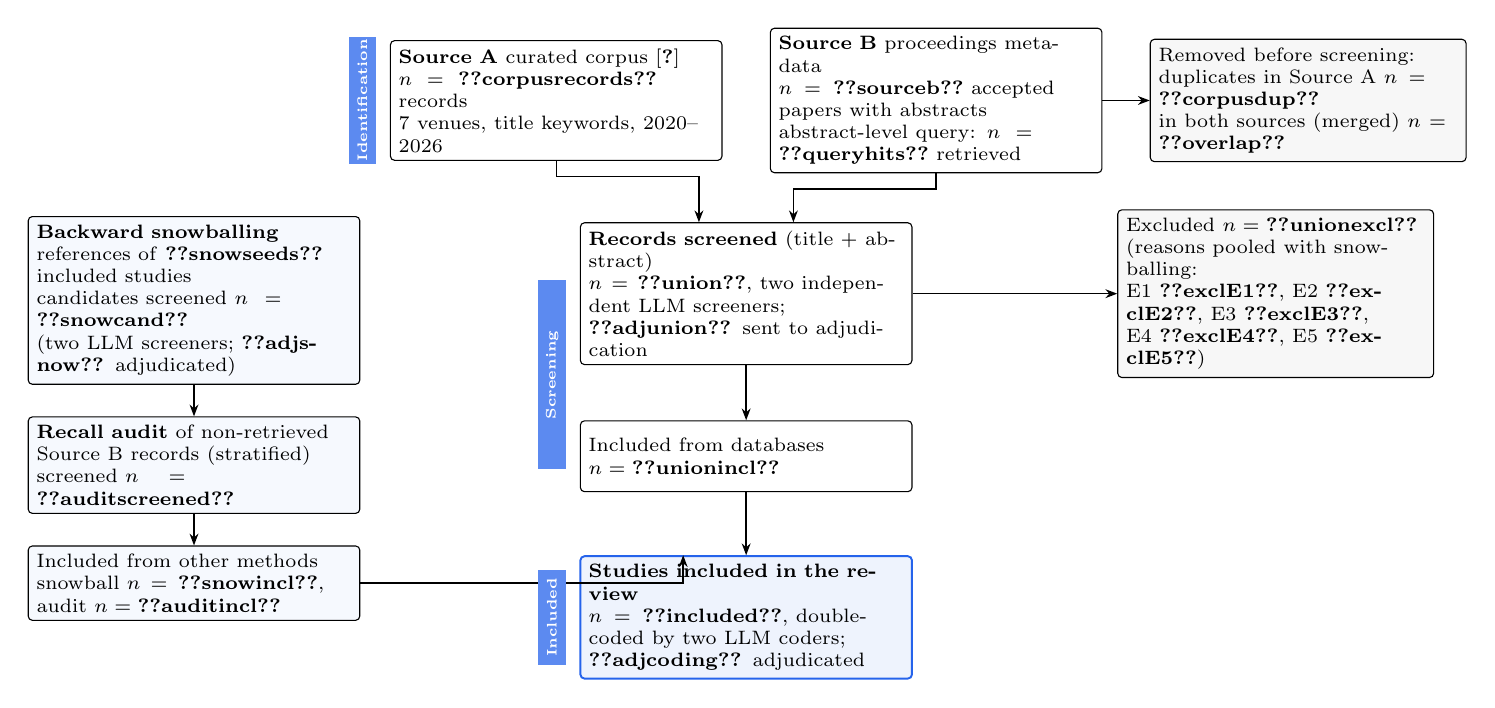
\begin{tikzpicture}[
  font=\scriptsize,
  box/.style={draw, rounded corners=1.5pt, align=left, text width=40mm, inner sep=3pt, minimum height=9mm},
  side/.style={draw, rounded corners=1.5pt, align=left, text width=38mm, inner sep=3pt, fill=black!3},
  oth/.style={draw, rounded corners=1.5pt, align=left, text width=40mm, inner sep=3pt, fill=nsblue!4},
  inc/.style={box, draw=nsblue, fill=nsblue!8, line width=0.7pt},
  stage/.style={fill=nsblue!75, text=white, font=\tiny\bfseries, minimum height=3.5mm, inner sep=1pt, rotate=90, anchor=center},
  arr/.style={-{Stealth[length=1.5mm]}, line width=0.5pt}]
% identification via databases
\node[box] (srcA) {\textbf{Source A} curated corpus~\cite{thakur2026repo}\\ $n=\cnt{corpusrecords}$ records\\ 7 venues, title keywords, 2020--2026};
\node[box, right=6mm of srcA] (srcB) {\textbf{Source B} proceedings metadata\\ $n=\cnt{sourceb}$ accepted papers with abstracts\\ abstract-level query: $n=\cnt{queryhits}$ retrieved};
\node[side, right=6mm of srcB] (dup) {Removed before screening:\\ duplicates in Source A $n=\cnt{corpusdup}$\\ in both sources (merged) $n=\cnt{overlap}$};
\node[box, below=7mm of $(srcA.south)!0.5!(srcB.south)$] (union) {\textbf{Records screened} (title + abstract)\\ $n=\cnt{union}$, two independent LLM screeners;\\ \cnt{adjunion} sent to adjudication};
\node[side, right=6mm of union, xshift=20mm] (ex) {Excluded $n=\cnt{unionexcl}$\\ (reasons pooled with snowballing:\\ E1 \cnt{exclE1}, E2 \cnt{exclE2}, E3 \cnt{exclE3},\\ E4 \cnt{exclE4}, E5 \cnt{exclE5})};
\node[box, below=7mm of union] (inu) {Included from databases\\ $n=\cnt{unionincl}$};
% other methods
\node[oth, below=7mm of srcA, xshift=-46mm] (snow) {\textbf{Backward snowballing}\\ references of \cnt{snowseeds} included studies\\ candidates screened $n=\cnt{snowcand}$\\ (two LLM screeners; \cnt{adjsnow} adjudicated)};
\node[oth, below=4mm of snow] (aud) {\textbf{Recall audit} of non-retrieved\\ Source B records (stratified)\\ screened $n=\cnt{auditscreened}$};
\node[oth, below=4mm of aud] (oi) {Included from other methods\\ snowball $n=\cnt{snowincl}$, audit $n=\cnt{auditincl}$};
\node[inc, below=8mm of inu] (all) {\textbf{Studies included in the review}\\ $n=\cnt{included}$, double-coded by two LLM coders;\\ \cnt{adjcoding} adjudicated};
\draw[arr] (srcA.south) -- ++(0,-2mm) -| ([xshift=-6mm]union.north);
\draw[arr] (srcB.south) -- ++(0,-2mm) -| ([xshift=6mm]union.north);
\draw[arr] (srcB) -- (dup);
\draw[arr] (union) -- (ex);
\draw[arr] (union) -- (inu);
\draw[arr] (inu) -- (all);
\draw[arr] (snow) -- (aud);
\draw[arr] (aud) -- (oi);
\draw[arr] (oi.east) -| ([xshift=-8mm]all.north);
\node[stage, minimum width=12mm] at ($(srcA.west)+(-3.5mm,0)$) {Identification};
\node[stage, minimum width=24mm] at ($($(union.west)!0.5!(inu.west)$)+(-3.5mm,0)$) {Screening};
\node[stage, minimum width=12mm] at ($(all.west)+(-3.5mm,0)$) {Included};
\end{tikzpicture}
\caption{PRISMA-ScR flow of evidence sources. Source A is the curated corpus (title-keyword collection); Source B is the accepted-paper metadata of eight venues, searched on title and abstract. All screening and coding decisions were made by LLM-based reviewers under protocol v2 (Section~\ref{sec:method-ai}).}
\label{fig:prisma}
\end{figure*}


Figure~\ref{fig:prisma} shows the flow. The union of the two sources contained \cnt{union} records, of which \cnt{unionincl} were included. Snowballing added \cnt{snowincl} studies from \cnt{snowcand} candidates, and the recall audit added \cnt{auditincl}, for a total of \cnt{included} included studies. Of the studies included from the union, \cnt{unioninclsearchonly} were found only by the abstract-level search and \cnt{unioninclcorpusonly} only by the curated corpus. Neither source alone would have sufficed: Source A is a title-keyword collection, and Source B does not cover AAAI 2020 and 2026, IJCAI 2025, TMLR or TPAMI.

\begin{table}[t]
\centering
\caption{Reasons for exclusion (union and snowball records). Each excluded record has the single most fundamental code.}
\label{tab:exclusions}
\footnotesize
\begin{tabular}{@{}lp{0.68\columnwidth}r@{}}
\toprule
Code & Reason & $n$ \\
\midrule
E3 & No interacting explicit symbolic component (R2--R6) & 1,197 \\
E1 & No language model (rule R1) & 577 \\
E4 & Not an archival research paper in scope & 27 \\
E5 & Survey, overview or position paper & 25 \\
E2 & Language model only as baseline, background or frozen encoder & 23 \\
\midrule
& Total excluded (union and snowball) & 1,849 \\
\bottomrule
\end{tabular}

\end{table}

\textbf{Exclusions.} The most frequent reason is E3, no interacting explicit symbolic component (Table~\ref{tab:exclusions}). The query is broad by design, so it retrieves many papers that use ``symbolic'', ``formal'' or ``program'' in a sense the protocol excludes: chain-of-thought prompting described as symbolic reasoning, retrieval of knowledge-graph triples, generic tool use, and code generation judged only by unit tests (rules R3--R6). E1 removes models trained from scratch on synthetic symbolic data and papers whose ``transformer'' is not a language model (R1).

\begin{table}[t]
\centering
\caption{Agreement between independent LLM reviewers before adjudication. Screening agreement is over three categories (include, exclude, unsure).}
\label{tab:agreement}
\footnotesize
\begin{tabular}{@{}lrrr@{}}
\toprule
Decision & $n$ & Agreement (\%) & $\kappa$ \\
\midrule
\multicolumn{4}{@{}l}{\textit{Screening (include / exclude / unsure)}} \\
\quad Union records & 2,130 & 92.9 & 0.85 \\
\quad Snowball candidates & 374 & 94.4 & 0.82 \\
\multicolumn{4}{@{}l}{\textit{Coding of included studies}} \\
\quad Architecture & 659 & 87.3 & 0.84 \\
\quad Check strength & 659 & 90.7 & 0.86 \\
\quad Domain & 659 & 90.3 & 0.89 \\
\quad Formalism & 659 & 91.5 & 0.90 \\
\quad Faithfulness reported & 659 & 90.4 & 0.71 \\
\bottomrule
\end{tabular}

\end{table}

\textbf{Agreement.} Table~\ref{tab:agreement} reports agreement between the two independent LLM screeners and between the two coders. On the union, the screeners agreed on \cnt{agreeunion}\% of records over three categories ($\kappa=\cnt{kappaunion}$). On include versus not include they agreed on \cnt{agreeunionincl}\% ($\kappa=\cnt{kappaunionincl}$). \cnt{unsureunion} records had at least one \texttt{unsure} decision; together with the conflicts, \cnt{adjunion} records went to adjudication, and \cnt{adjinclunion} of these were included. Coding agreement ranged from $\kappa=\cnt{kappafaith}$ for faithfulness reporting to $\kappa=\cnt{kappaform}$ for formalism, with $\kappa=\cnt{kappaarch}$ for architecture. As Section~\ref{sec:method-ai} explains, these figures measure the consistency of independent model runs under explicit rules, not human reliability.

\textbf{Recall.} The audit found \cnt{auditlmx} eligible studies among \cnt{auditlmn} sampled records with language-model terms only, \cnt{auditsymx} among \cnt{auditsymn} with symbolic terms only, and \cnt{auditneix} among \cnt{auditnein} with neither. Scaled to the strata, this suggests that about \cnt{missedpoint} eligible studies in Source B were not retrieved (95\% interval \cnt{missedlo}--\cnt{missedhi}). Search recall is therefore estimated at \cnt{recallpoint}, with a 95\% interval of \cnt{recalllo}--\cnt{recallhi}. The lower bound is driven by the large neither stratum, where the sample found no eligible study. If that stratum is assumed to contain none, the interval narrows to \cnt{recallsenslo}--\cnt{recallsenshi}. The studies the audit found illustrate what the query misses: abstracts that describe a model-checker repair loop, an optimisation-modelling pipeline, interpreter-generated training targets or Prolog-generated training data without the query's symbolic vocabulary. We therefore read every count in this paper as a count of the \emph{retrievable} literature, which is a large but incomplete share. The proportions and associations we report are robust to missing studies only if the missed studies resemble the found ones. The audit gives no indication otherwise, but its sample is small.

\textbf{Known-item check.} A reviewer of the pilot named nine studies that the pilot missed: PAL~\cite{gao2023pal}, SatLM~\cite{ye2023satlm}, Binder~\cite{cheng2023binding}, Draft-Sketch-Prove~\cite{jiang2023draft}, LeanDojo~\cite{yang2023leandojo}, Thor~\cite{jiang2022thor}, autoformalisation with LLMs~\cite{wu2022autoformalization}, LLM-SR~\cite{shojaee2025sr} and Lean-STaR~\cite{lin2025lean}. All nine were retrieved and included.

\textbf{Venues and years.} ICLR (\cnt{ICLR} studies), ICML (\cnt{ICML}) and NeurIPS (\cnt{NeurIPS}) contribute most studies, followed by the NLP venues EMNLP (\cnt{EMNLP}), ACL (\cnt{ACL}) and NAACL (\cnt{NAACL}), and by AAAI (\cnt{AAAI}) and IJCAI (\cnt{IJCAI}). TMLR and TPAMI contribute \cnt{TMLR} and \cnt{TPAMI}, because they are covered only by the title-keyword corpus (Table~\ref{tab:sources}). By year, the included studies number \cnt{y2020} (2020), \cnt{y2021}, \cnt{y2022}, \cnt{y2023}, \cnt{y2024}, \cnt{y2025} and \cnt{y2026} (2026, partial). Section~\ref{sec:trends} normalises these counts.

\section{RQ1: Integration Architectures}
\label{sec:taxonomy}

% Schematic of the seven integration architectures (A1--A7).
\begin{figure*}[t]
\centering
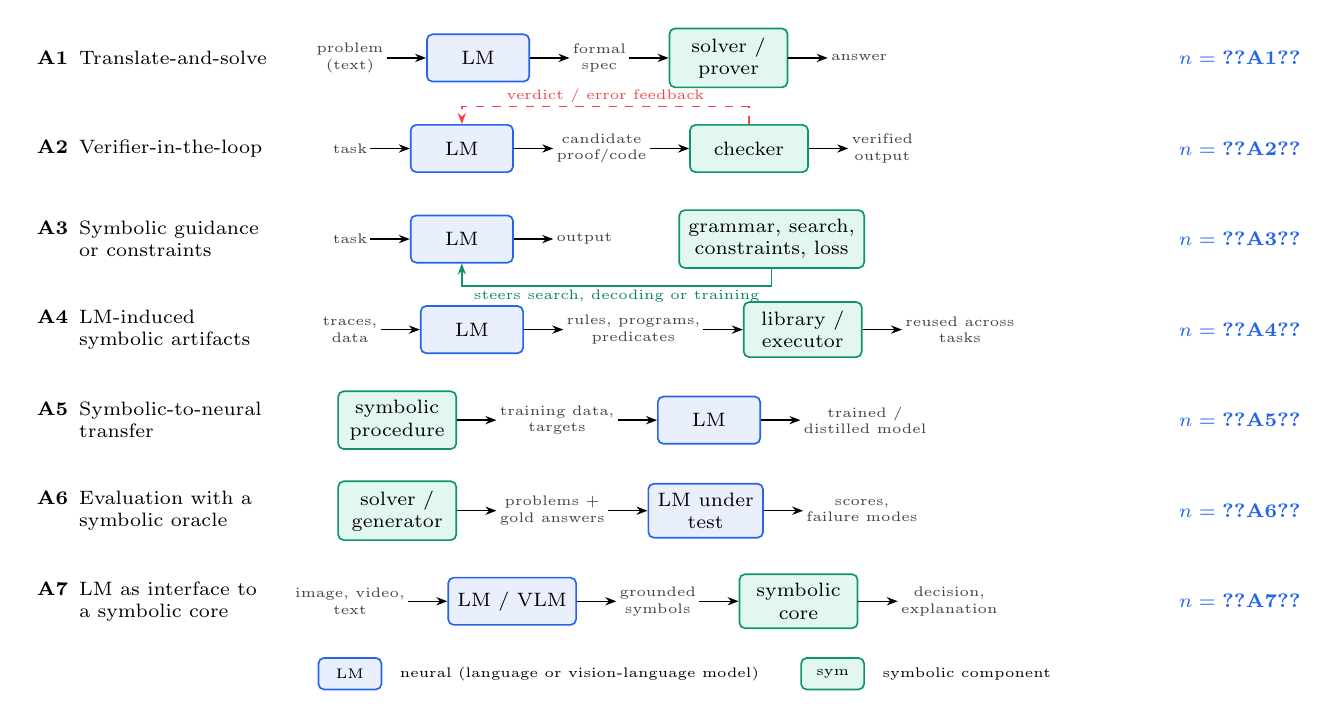
\begin{tikzpicture}[
  font=\scriptsize,
  lab/.style={align=left, anchor=west, text width=33mm},
  lm/.style={draw=nsblue, fill=nsblue!10, rounded corners=2pt, minimum height=6mm, minimum width=13mm, align=center, line width=0.6pt},
  sym/.style={draw=A3c!80!black, fill=A3c!12, rounded corners=2pt, minimum height=6mm, minimum width=15mm, align=center, line width=0.6pt},
  dat/.style={align=center, text=black!75, font=\tiny, inner sep=1pt},
  arr/.style={-{Stealth[length=1.4mm]}, line width=0.5pt},
  fb/.style={-{Stealth[length=1.4mm]}, line width=0.5pt, dashed, draw=A5c},
  cnt/.style={anchor=east, font=\scriptsize\bfseries, text=nsblue}]
\def\rowgap{11.5mm}
\def\xs{41mm}
% ---- A1
\node[lab] (l1) at (0,0) {\textbf{A1}\enspace Translate-and-solve};
\node[dat] (a1i) at (\xs,0) {problem\\(text)};
\node[lm, right=5mm of a1i] (a1m) {LM};
\node[dat, right=5mm of a1m] (a1f) {formal\\spec};
\node[sym, right=5mm of a1f] (a1s) {solver /\\prover};
\node[dat, right=5mm of a1s] (a1o) {answer};
\draw[arr] (a1i)--(a1m); \draw[arr] (a1m)--(a1f); \draw[arr] (a1f)--(a1s); \draw[arr] (a1s)--(a1o);
\node[cnt] at (16.3,0) {$n=\cnt{A1}$};
% ---- A2
\node[lab] (l2) at (0,-\rowgap) {\textbf{A2}\enspace Verifier-in-the-loop};
\node[dat] (a2i) at (\xs,-\rowgap) {task};
\node[lm, right=5mm of a2i] (a2m) {LM};
\node[dat, right=5mm of a2m] (a2f) {candidate\\proof/code};
\node[sym, right=5mm of a2f] (a2s) {checker};
\node[dat, right=5mm of a2s] (a2o) {verified\\output};
\draw[arr] (a2i)--(a2m); \draw[arr] (a2m)--(a2f); \draw[arr] (a2f)--(a2s); \draw[arr] (a2s)--(a2o);
\draw[fb] (a2s.north) -- ++(0,2.2mm) -| node[pos=0.25, above, font=\tiny, text=A5c, inner sep=1pt] {verdict / error feedback} (a2m.north);
\node[cnt] at (16.3,-\rowgap) {$n=\cnt{A2}$};
% ---- A3
\node[lab] (l3) at (0,-2*\rowgap) {\textbf{A3}\enspace Symbolic guidance\\\phantom{\textbf{A3}}\enspace or constraints};
\node[dat] (a3i) at (\xs,-2*\rowgap) {task};
\node[lm, right=5mm of a3i] (a3m) {LM};
\node[dat, right=5mm of a3m] (a3o) {output};
\node[sym, right=8mm of a3o] (a3s) {grammar, search,\\constraints, loss};
\draw[arr] (a3i)--(a3m); \draw[arr] (a3m)--(a3o);
\draw[arr, draw=A3c!80!black] (a3s.south) -- ++(0,-2.2mm) -| node[pos=0.25, below, font=\tiny, text=A3c!70!black, inner sep=1pt] {steers search, decoding or training} (a3m.south);
\node[cnt] at (16.3,-2*\rowgap) {$n=\cnt{A3}$};
% ---- A4
\node[lab] (l4) at (0,-3*\rowgap) {\textbf{A4}\enspace LM-induced\\\phantom{\textbf{A4}}\enspace symbolic artifacts};
\node[dat] (a4i) at (\xs,-3*\rowgap) {traces,\\data};
\node[lm, right=5mm of a4i] (a4m) {LM};
\node[dat, right=5mm of a4m] (a4f) {rules, programs,\\predicates};
\node[sym, right=5mm of a4f] (a4s) {library /\\executor};
\node[dat, right=5mm of a4s] (a4o) {reused across\\tasks};
\draw[arr] (a4i)--(a4m); \draw[arr] (a4m)--(a4f); \draw[arr] (a4f)--(a4s); \draw[arr] (a4s)--(a4o);
\node[cnt] at (16.3,-3*\rowgap) {$n=\cnt{A4}$};
% ---- A5
\node[lab] (l5) at (0,-4*\rowgap) {\textbf{A5}\enspace Symbolic-to-neural\\\phantom{\textbf{A5}}\enspace transfer};
\node[sym] (a5s) at ($(\xs,-4*\rowgap)+(6mm,0)$) {symbolic\\procedure};
\node[dat, right=5mm of a5s] (a5f) {training data,\\targets};
\node[lm, right=5mm of a5f] (a5m) {LM};
\node[dat, right=5mm of a5m] (a5o) {trained /\\distilled model};
\draw[arr] (a5s)--(a5f); \draw[arr] (a5f)--(a5m); \draw[arr] (a5m)--(a5o);
\node[cnt] at (16.3,-4*\rowgap) {$n=\cnt{A5}$};
% ---- A6
\node[lab] (l6) at (0,-5*\rowgap) {\textbf{A6}\enspace Evaluation with a\\\phantom{\textbf{A6}}\enspace symbolic oracle};
\node[sym] (a6s) at ($(\xs,-5*\rowgap)+(6mm,0)$) {solver /\\generator};
\node[dat, right=5mm of a6s] (a6f) {problems +\\gold answers};
\node[lm, right=5mm of a6f] (a6m) {LM under\\test};
\node[dat, right=5mm of a6m] (a6o) {scores,\\failure modes};
\draw[arr] (a6s)--(a6f); \draw[arr] (a6f)--(a6m); \draw[arr] (a6m)--(a6o);
\node[cnt] at (16.3,-5*\rowgap) {$n=\cnt{A6}$};
% ---- A7
\node[lab] (l7) at (0,-6*\rowgap) {\textbf{A7}\enspace LM as interface to\\\phantom{\textbf{A7}}\enspace a symbolic core};
\node[dat] (a7i) at (\xs,-6*\rowgap) {image, video,\\text};
\node[lm, right=5mm of a7i] (a7m) {LM / VLM};
\node[dat, right=5mm of a7m] (a7f) {grounded\\symbols};
\node[sym, right=5mm of a7f] (a7s) {symbolic\\core};
\node[dat, right=5mm of a7s] (a7o) {decision,\\explanation};
\draw[arr] (a7i)--(a7m); \draw[arr] (a7m)--(a7f); \draw[arr] (a7f)--(a7s); \draw[arr] (a7s)--(a7o);
\node[cnt] at (16.3,-6*\rowgap) {$n=\cnt{A7}$};
% legend
\node[lm, minimum width=8mm, minimum height=4mm, font=\tiny] (k1) at (\xs,-6.8*\rowgap) {LM};
\node[right=1mm of k1, font=\tiny] (k1t) {neural (language or vision-language model)};
\node[sym, minimum width=8mm, minimum height=4mm, font=\tiny, right=4mm of k1t] (k2) {sym};
\node[right=1mm of k2, font=\tiny] {symbolic component};
\end{tikzpicture}
\caption{The seven integration architectures identified in the \cnt{included} included studies, with the number of studies coded under each. Blue boxes are learned models; green boxes are symbolic components. Dashed arrows denote feedback from the symbolic component to the model.}
\label{fig:architectures}
\end{figure*}


The \cnt{included} studies fall into seven architectures (Fig.~\ref{fig:architectures}). Checker-in-the-loop designs dominate (A2, \cnt{A2} studies, \cnt{A2pct}\%), followed by symbolic-oracle evaluations (A6, \cnt{A6}), translate-and-solve pipelines (A1, \cnt{A1}) and symbolic guidance (A3, \cnt{A3}). Symbolic-to-neural transfer (A5, \cnt{A5}), model-induced artifacts (A4, \cnt{A4}) and model-as-interface designs (A7, \cnt{A7}) are less common. Across all studies, the symbolic side gives an exact verdict on the final output in \cnt{exact} studies, an empirical check in \cnt{empirical}, and no check in \cnt{none}. The architectures differ in where trust is placed, which determines what a system can guarantee.

\textbf{A2: Checker-in-the-loop (\cnt{A2}).} A checker or executor returns verdicts that select, repair, filter or reward model outputs. The category splits by check strength.
\begin{itemize}
  \item \emph{Exact} (\cnt{A2exact} studies). Here the proof assistant's acceptance is a guarantee relative to the formal statement. Typical approaches are proof search~\cite{lample2022hypertree,jiang2022thor,yang2023leandojo,xin2025bfs}, proof-assistant feedback for reinforcement learning~\cite{xin2025deepseek,dong2025stp,lin2026goedel}, and draft-and-prove pipelines~\cite{jiang2023draft,cao2025reviving,varambally2026hilbert}. Verification-aware code generation in Dafny or Verus~\cite{aggarwal2025alphaverus,yang2026exverus}, model-checking repair loops~\cite{agrawal2025specmas} and SAT-certified reasoning rewards~\cite{liu2025saturn} belong here too.
  \item \emph{Empirical} (\cnt{A2empirical} studies). Here the check can pass a wrong output: execution feedback for code and programming by example~\cite{ni2023lever,wang2024hypothesis,lee2025program}, solver feedback in optimisation modelling~\cite{ahmaditeshnizi2024optimus,chen2025solver}, data fit in LLM-guided equation search~\cite{shojaee2025sr,grayeli2024symbolic}, and simulator or environment success in embodied agents~\cite{ma2024eureka,mahdavi2024leveraging}.
\end{itemize}
Because A2 thus mixes sound verification with tests and data fit, we report the two kinds separately and restrict statements about guarantees to exact checks.

\textbf{A6: Symbolic-oracle evaluation (\cnt{A6}).} Benchmarks whose problems are generated, or whose answers are certified, by a symbolic system. Examples are solver-generated logic puzzles~\cite{lin2025zebralogic,wei2025satbench}, prover-checked first-order reasoning~\cite{qi2025large,han2024folio}, and planning benchmarks with formal validators~\cite{zuo2025planetarium,kokel2025acpbench}. Formal-mathematics and verification benchmarks~\cite{zheng2022minif2f,tsoukalas2024putnambench,hu2025minictx,ye2026verina} and symbolic perturbations of mathematical word problems~\cite{mirzadeh2025gsm} also belong here. Most A6 studies certify answers empirically (\cnt{A6empirical}), for example by answer matching against a generator. Only \cnt{A6exact} use a sound checker.

\textbf{A1: Translate-and-solve (\cnt{A1}).} The model writes a formal representation once and an engine computes the answer, so correctness reduces to the faithfulness of the translation. Program-aided reasoning~\cite{gao2023pal,gou2024tora,wang2024mathcoder} and binding language models to symbolic languages~\cite{cheng2023binding} are the largest group. Others translate text to first-order logic or SAT~\cite{olausson2023linc,ye2023satlm,kesseli2025logic}, answer-set programs~\cite{alviano2025integrating,santana2024automatic}, planning languages~\cite{hao2025planning,huang2025planning} or optimisation models~\cite{astorga2025autoformulation,yang2025optibench}. By construction, A1 pipelines do not check the model's formalisation (all \cnt{A1none} are coded \texttt{none}), which is why reporting formalisation faithfulness matters (Section~\ref{sec:evaluation}).

\textbf{A3: Symbolic guidance (\cnt{A3}).} Symbolic structure steers generation without judging it. Examples include constrained decoding with grammars and automata~\cite{scholak2021picard,wang2023grammar,beurerkellner2024guiding,banerjee2025crane}, logical decoding constraints~\cite{lu2021neurologic,lu2022neurologic,zhang2023tractable}, and static or dataflow analysis that guides code models~\cite{mukherjee2021neural,wei2023typet5,li2025dataflow}. Context-free surrogates of model proposals that guide enumerative synthesis~\cite{barke2024hysynth} and neurosymbolic training losses~\cite{ahmed2023pseudo} also belong here.

\textbf{A5: Symbolic-to-neural transfer (\cnt{A5}).} Symbolic procedures generate training data or signal offline, and the model runs without them: synthetic logic corpora~\cite{clark2020transformers,morishita2023learning,morishita2024enhancing}, formal theorem--proof data~\cite{huang2024mustard,ying2024lean,wu2025alchemy}, solver-generated mathematics~\cite{li2024neuro}, interpreter-generated execution traces~\cite{li2025codeio,wang2026stepcodereasoner}, and consistency losses against a rule base~\cite{calanzone2025logically}.

\textbf{A4: LM-induced artifacts (\cnt{A4}).} The model writes rules, programs, predicates or reward machines that are stored and reused, but no symbolic checker filters them; libraries that are filtered by tests or verification are A2 under the decision tree. Examples include programmatic world models~\cite{tang2024worldcoder,piriyakulkij2025poe}, invented predicates and planning domains for robots~\cite{liang2025visualpredicator,liang2026exopredicator,ye2025unidomain}, interpretable rule libraries~\cite{wang2025large,zhang2025ruag}, and reward functions or reward machines~\cite{xie2024text2reward,castanyer2026arm}.

\textbf{A7: LM as interface (\cnt{A7}).} A language or vision-language model grounds perception or produces explanations, and a symbolic core decides. Examples include logic-rule latent models over vision-language judgements~\cite{he2026unveiling}, robustness of vision-language reasoning with a symbolic executor~\cite{chen2026vlms}, programmable neurosymbolic learning frameworks~\cite{naik2025dolphin}, and knowledge-enhanced logical guardrails~\cite{kang2025r2}.

\subsection{Relation to existing integration taxonomies}
\label{sec:taxonomy-relations}
Table~\ref{tab:taxmap} relates the architectures to Kautz's integration types~\cite{kautz2022third} and to the perspectives of Yang et al.~\cite{yang2025neuro}. The correspondence is approximate, but it shows what the finer scheme adds. Kautz's Neuro|Symbolic pipeline covers A1, A4 and A7, which differ in what the symbolic side receives: a whole problem, a reusable artifact or grounded percepts. Yang et al.'s LLM+Symbolic perspective merges A2, where the symbolic side judges, with A3, where it only steers. The check-strength attribute adds a second distinction no earlier scheme records: whether that judgement is sound.

\begin{table}[t]
\centering
\caption{Approximate correspondence with existing taxonomies.}
\label{tab:taxmap}
\footnotesize
\begin{tabularx}{\columnwidth}{@{}l X X@{}}
\toprule
Ours & Kautz~\cite{kautz2022third} & Yang et al.~\cite{yang2025neuro} \\
\midrule
A1 & Neuro|Symbolic & LLM$\rightarrow$Symbolic \\
A2 & Neuro|Symbolic with feedback & LLM+Symbolic \\
A3 & Symbolic[Neuro] (search); Neuro$_\text{Symbolic}$ (loss) & LLM+Symbolic; Symbolic$\rightarrow$LLM \\
A4 & Neuro|Symbolic & LLM$\rightarrow$Symbolic \\
A5 & Neuro:Symbolic$\rightarrow$Neuro & Symbolic$\rightarrow$LLM \\
A6 & -- (evaluation) & -- \\
A7 & Neuro|Symbolic & LLM$\rightarrow$Symbolic \\
\bottomrule
\end{tabularx}
\end{table}

\section{RQ2: Domains, Formalisms and Their Association with Architecture}
\label{sec:domains}

\begin{table*}[t]
\centering
\caption{Task domain $\times$ integration architecture, with check strength (ex.\ = exact, emp.\ = empirical). Shading is proportional to the count.}
\label{tab:domainarch}
\footnotesize
\setlength{\tabcolsep}{3.2pt}
\begin{tabular}{@{}lcccccccr@{}}
\toprule
Domain & A1 & A2 & A3 & A4 & A5 & A6 & A7 & $\Sigma$ \\
\midrule
D2: Logical \& deductive reasoning & \cellcolor{nsblue!70}8 & \cellcolor{nsblue!17}1 & \cellcolor{nsblue!32}3 & \textcolor{black!35}{0} & \textcolor{black!35}{0} & \cellcolor{nsblue!40}4 & \textcolor{black!35}{0} & 16 \\
D1: Formal theorem proving \& autoformalization & \cellcolor{nsblue!17}1 & \cellcolor{nsblue!55}6 & \cellcolor{nsblue!40}4 & \cellcolor{nsblue!17}1 & \textcolor{black!35}{0} & \cellcolor{nsblue!25}2 & \textcolor{black!35}{0} & 14 \\
D6: Vision-language \& multimodal reasoning & \cellcolor{nsblue!17}1 & \textcolor{black!35}{0} & \textcolor{black!35}{0} & \cellcolor{nsblue!32}3 & \cellcolor{nsblue!17}1 & \cellcolor{nsblue!32}3 & \cellcolor{nsblue!40}4 & 12 \\
D5: Embodied planning \& agents & \textcolor{black!35}{0} & \cellcolor{nsblue!25}2 & \cellcolor{nsblue!25}2 & \cellcolor{nsblue!47}5 & \cellcolor{nsblue!17}1 & \textcolor{black!35}{0} & \cellcolor{nsblue!17}1 & 11 \\
D3: Program synthesis \& structured-data reasoning & \textcolor{black!35}{0} & \cellcolor{nsblue!25}2 & \cellcolor{nsblue!55}6 & \cellcolor{nsblue!25}2 & \textcolor{black!35}{0} & \textcolor{black!35}{0} & \textcolor{black!35}{0} & 10 \\
D7: Language modelling, knowledge \& data synthesis & \textcolor{black!35}{0} & \textcolor{black!35}{0} & \cellcolor{nsblue!25}2 & \cellcolor{nsblue!25}2 & \cellcolor{nsblue!25}2 & \textcolor{black!35}{0} & \textcolor{black!35}{0} & 6 \\
D4: Symbolic regression \& scientific discovery & \textcolor{black!35}{0} & \cellcolor{nsblue!25}2 & \cellcolor{nsblue!17}1 & \cellcolor{nsblue!17}1 & \textcolor{black!35}{0} & \textcolor{black!35}{0} & \textcolor{black!35}{0} & 4 \\
\midrule
$\Sigma$ & 10 & 13 & 18 & 14 & 4 & 9 & 5 & 73 \\
\bottomrule
\end{tabular}

\end{table*}

Table~\ref{tab:domainarch} cross-tabulates domains and architectures. Architecture is moderately associated with domain: Cram\'er's $V=\cnt{Vall}$, bias-corrected $V=\cnt{Vcall}$~\cite{bergsma2013bias}, against a mean of \cnt{Vnullall} under the permutation null; no permuted table reached the observed $\chi^2$ in \cnt{npermall} shuffles ($p<0.001$). Part of an association like this could be definitional: theorem proving is defined by proof assistants, and vision-language studies might gravitate to perception interfaces. Excluding these two domains (D1 and D6) leaves the association unchanged (bias-corrected $V=\cnt{Vcsens}$, null mean \cnt{Vnullsens}). Formalism is, as expected, much more strongly tied to domain (bias-corrected $V=\cnt{Vcform}$). In the pilot, a smaller sample overstated the architecture--domain association; with \cnt{included} studies, ``moderate'' is the accurate description.

\begin{table}[t]
\centering
\caption{Symbolic formalisms.}
\label{tab:formalism}
\footnotesize
\begin{tabular}{@{}llr@{}}
\toprule
Code & Symbolic formalism & $n$ \\
\midrule
F1 & Logic (FOL, ASP, Prolog, constraints) & 22 \\
F2 & Proof assistants (Lean, Isabelle) & 14 \\
F3 & Programs \& DSLs & 13 \\
F7 & Other (automata, static analysis, solvers) & 9 \\
F5 & Knowledge graphs, rules \& scene graphs & 6 \\
F6 & Planning \& temporal logic & 5 \\
F4 & Symbolic expressions & 4 \\
\bottomrule
\end{tabular}

\end{table}

\subsection{Theorem proving and autoformalisation (D1, \cnt{D1} studies)}
D1 is the domain of exact checking: \cnt{D1exact} of its \cnt{D1} studies receive a sound verdict, almost all from Lean or Isabelle. Checker-in-the-loop is the dominant architecture (\cnt{D1A2}). Its lineage runs from proof search with pretrained tactic models~\cite{han2022proof,lample2022hypertree,polu2023formal} through hammers and premise selection~\cite{jiang2022thor,mikua2024magnushammer} and retrieval-augmented provers~\cite{yang2023leandojo} to reinforcement learning from proof-assistant feedback~\cite{xin2025deepseek,lin2026goedel,xin2026scaling}. Recent work adds self-play conjecturing~\cite{dong2025stp,wilf2026propose}, growing lemma libraries~\cite{wang2024lego}, agentic repair~\cite{requena2026minimal,ospanov2025apollo} and recursive informal-to-formal decomposition~\cite{jiang2023draft,varambally2026hilbert}. Autoformalisation forms a second strand~\cite{wu2022autoformalization,li2024autoformalize,chen2026reform,cabral2026proofflow}, and formal software verification in Verus, Dafny and Isabelle a third~\cite{wu2024lemur,lin2024fvel,aggarwal2025alphaverus,chen2025automated}. D1 also has the most evaluation studies after D2 (\cnt{D1A6}), which increasingly test the benchmarks themselves~\cite{ospanov2025minif2f,ammanamanchi2026faults,poiroux2025reliable}. Section~\ref{sec:evaluation} shows what the shared benchmark reveals.

\subsection{Logical and deductive reasoning (D2, \cnt{D2} studies)}
D2 is the evaluation-heavy domain: \cnt{D2A6} of its studies are symbolic-oracle benchmarks. They use solvers, provers and logic programs to generate problems with certified answers at controlled difficulty~\cite{saparov2023language,lin2025zebralogic,qi2025large,wei2025satbench,xu2026socrates}, or to measure properties beyond accuracy such as efficiency~\cite{opedal2025language} and self-verification~\cite{stechly2025self}. Among methods, checker-in-the-loop designs (\cnt{D2A2}) outnumber translate-and-solve pipelines (\cnt{D2A1}). The translate-and-solve line formalises text into first-order logic, SAT or answer-set programs for an external engine~\cite{olausson2023linc,ye2023satlm,alviano2025integrating,jurayj2026language}. The checker line verifies or repairs the model's reasoning with a prover or solver~\cite{quan2024verification,ryu2025divide,feng2026vericot,schrader2026solver}. Synthetic logic corpora that train models to reason form a third line (A5, \cnt{D2A5})~\cite{clark2020transformers,morishita2024enhancing,wang2025logictree}. Checks in D2 are mostly empirical (\cnt{D2empirical}) rather than exact (\cnt{D2exact}), because the checker usually certifies consistency or the answer rather than the translation.

\subsection{Program synthesis and structured data (D3, \cnt{D3} studies)}
D3 spans three architectures. Execution-checked synthesis (A2, \cnt{D3A2}) covers programming by example, abstraction learning and LLM-driven algorithm or heuristic design~\cite{wang2024hypothesis,li2025combining,stengeleskin2024regal,liu2024evolution,ye2024reevo}. Translate-and-solve (\cnt{D3A1}) dominates table question answering~\cite{cheng2023binding,cao2023api,abhyankar2025h}. Symbolic guidance (\cnt{D3A3}) collects grammar-constrained decoding and static analysis~\cite{scholak2021picard,wang2023grammar,wei2023typet5,barke2024hysynth}. Exact checks are rare (\cnt{D3exact}) and come from verified transpilation and formal equivalence checking~\cite{bhatia2024verified,lee2024guess}.

\subsection{Mathematical problem solving (D7, \cnt{D7} studies)}
D7 is where program-aided reasoning lives. Translate-and-solve (\cnt{D7A1}) covers PAL-style programs~\cite{gao2023pal}, tool-integrated reasoning agents and their training data~\cite{gou2024tora,wang2024mathcoder,toshniwal2024openmathinstruct}, and optimisation modelling, in which the model writes a solver model~\cite{astorga2025autoformulation,yang2025optibench}. Checker-in-the-loop (\cnt{D7A2}) adds execution feedback and verification during training or inference~\cite{zhou2024solving,xiong2025building,feng2026retool}. It also adds formal checks of informal solutions: autoformalising a model's answer and verifying it in Lean~\cite{zhou2024don,yao2025fans,ospanov2026hermes}. Symbolic perturbation benchmarks show how brittle informal mathematical reasoning is~\cite{mirzadeh2025gsm,opedal2025mathgap}.

\subsection{Embodied planning and agents (D5, \cnt{D5} studies)}
D5 is the domain of reusable artifacts. A4 is more common here (\cnt{D5A4}) than in any other domain: models induce PDDL domains, predicates, programmatic world models and reward machines that agents reuse~\cite{tang2024worldcoder,liang2026exopredicator,liang2025visualpredicator,ye2025unidomain,castanyer2026arm}. Checker-in-the-loop (\cnt{D5A2}) uses planners, simulators and execution to validate plans or code-as-policies~\cite{silver2024generalized,mahdavi2024leveraging,ahn2025reliable}. Translate-and-solve (\cnt{D5A1}) hands formalised tasks to classical planners or solvers~\cite{hao2025planning,huang2025planning}. Exact checks are rare (\cnt{D5exact}), because success in an environment is an empirical signal.

\subsection{Language, knowledge and data (D8, \cnt{D8} studies)}
D8 is the stronghold of symbolic guidance (\cnt{D8A3}): constrained decoding with logic, grammars and automata~\cite{lu2021neurologic,zhang2023tractable,beurerkellner2024guiding,ahmed2025controllable,suresh2025dingo}, semantic parsing~\cite{shin2021constrained,herzig2021span} and language models augmented with symbolic functions~\cite{demeter2020just}. Data synthesis and consistency training against rules form the A5 group (\cnt{D8A5})~\cite{calanzone2025logically,li2025codeio,jiang2026procedural}.

\subsection{Vision-language and multimodal (D6, \cnt{D6} studies)}
D6 is spread across architectures. Translate-and-solve (\cnt{D6A1}) covers visual programming and program-based question answering~\cite{subramanian2023modular,hsu2023s,kamali2026neptune}. Generated modules are filtered by execution in A2 (\cnt{D6A2})~\cite{chen2024genome,belouadi2024detikzify}. Perception interfaces to a symbolic core make up A7 (\cnt{D6A7})~\cite{naik2025dolphin,chen2026vlms,he2026unveiling}, and logic benchmarks make up A6~\cite{gao2023lora,xu2025muslr}. Grounding open-vocabulary symbols is a recurring motivation~\cite{kamali2025nesycoco,sinha2026concept}. No D6 study has an exact check.

\subsection{Symbolic regression and discovery (D4, \cnt{D4} studies)}
In D4 the model acts as a proposal operator inside an evolutionary or agentic equation search, and fit to data is the check (\cnt{D4A2} A2 studies, all empirical)~\cite{shojaee2025sr,grayeli2024symbolic,xia2026sr,pang2026deliberate}. Symbolic equivalence and concept libraries make the search more efficient~\cite{jiang2026egg,grayeli2024symbolic}. Benchmarks are new and few~\cite{shojaee2025srbench,zheng2026newtonbench}. Rule R1 excludes transformer models trained from scratch on synthetic equations, which is why this large adjacent literature is not counted here.

\subsection{Formalisms}
General-purpose programs (F3, \cnt{F3}) and logic (F1, \cnt{F1}) are the most common representations, followed by DSLs, grammars and static analysis (F7, \cnt{F7}) and proof assistants (F2, \cnt{F2}); see Table~\ref{tab:formalism}. Formalism tracks domain closely: \cnt{D1F2} of the \cnt{D1} D1 studies use a proof assistant, \cnt{D2F1} of the \cnt{D2} D2 studies use logic, and planning languages are concentrated in D5 (\cnt{D5F6} of \cnt{F6} studies).

\section{RQ3: Models, Engines, Benchmarks, Faithfulness and Reproducibility}
\label{sec:evaluation}

\begin{table}[t]
\centering
\caption{Language-model families, symbolic engines and benchmarks named in the abstracts of included studies (open-vocabulary extraction by two coders; a study counts if either coder listed it).}
\label{tab:entities}
\footnotesize
\begin{tabular}{@{}lr@{}}
\toprule
Named in abstract & Studies \\
\midrule
\multicolumn{2}{@{}l}{\textit{Language-model families (199 studies name one)}} \\
\quad GPT-4 family & 93 \\
\quad GPT-3/3.5, ChatGPT, Codex & 47 \\
\quad Llama family & 46 \\
\quad DeepSeek family & 29 \\
\quad Gemini/PaLM/Bard & 25 \\
\quad Specialised provers & 15 \\
\quad Claude & 13 \\
\quad BERT family & 11 \\
\quad Qwen family & 11 \\
\midrule
\multicolumn{2}{@{}l}{\textit{Symbolic engines (215 studies name one)}} \\
\quad Python interpreter/executor & 70 \\
\quad Lean & 62 \\
\quad Planners (PDDL) & 19 \\
\quad SAT/SMT (Z3, cvc5) & 17 \\
\quad Optimisation solvers (LP/MILP/CP) & 15 \\
\quad Isabelle & 13 \\
\quad Logic programming (Prolog, ASP, Datalog) & 9 \\
\quad Theorem provers (FOL) & 8 \\
\quad Dafny/Verus/Why3/F* & 8 \\
\midrule
\multicolumn{2}{@{}l}{\textit{Benchmarks (353 studies name one)}} \\
\quad miniF2F & 42 \\
\quad MATH & 16 \\
\quad ProofNet & 14 \\
\quad GSM8K & 12 \\
\quad ALFWorld & 8 \\
\quad PutnamBench & 8 \\
\quad HumanEval & 7 \\
\quad AIME & 6 \\
\quad WikiTableQuestions & 5 \\
\bottomrule
\end{tabular}

\end{table}

\textbf{What abstracts name.} Table~\ref{tab:entities} summarises the entities named in abstracts. The two coders agreed well on model families and benchmarks (mean Jaccard \cnt{jaclm} and \cnt{jacbenchmark}) and less well on engines (\cnt{jacengine}), so engine counts are approximate. Only \cnt{lmstudies} studies (\cnt{lmstudiespct}\%) name a model family in the abstract; the counts describe reporting in abstracts, not usage. Among them, GPT-4-family models are the most named (\cnt{lmGPT4}). Proprietary and open-weight families are used side by side: \cnt{lmprop} studies name a proprietary family and \cnt{lmopen} an open-weight one, while \cnt{lmproponly} name only proprietary families. The Python interpreter (\cnt{engPython}) and Lean (\cnt{engLean}) are the most named engines, which reflects the weight of program-aided reasoning and formal theorem proving.

\textbf{Benchmarks are fragmented.} \cnt{benchstudies} studies name at least one benchmark in the abstract, and together they name \cnt{benchdistinct} distinct benchmarks. Of these, \cnt{benchsingle} (\cnt{benchsinglepct}\%) are named by a single study, and only \cnt{benchfiveplus} are named by five or more. miniF2F is the only benchmark named by more than 20 studies (\cnt{benchminif2f}). This conclusion no longer depends on a fixed dictionary, because the vocabulary is open. Abstracts under-report benchmarks, though, so the true overlap is somewhat higher.

% miniF2F pass rates reported in abstracts of included studies (data/derived/plot_minif2f.csv).
\begin{figure}[t]
\centering
\begin{tikzpicture}
\begin{axis}[
  width=\columnwidth, height=52mm,
  xmin=2021.6, xmax=2026.5, ymin=20, ymax=105,
  xtick={2022,2023,2024,2025,2026},
  xticklabel style={font=\scriptsize, /pgf/number format/1000 sep={}},
  yticklabel style={font=\scriptsize},
  ylabel={Reported miniF2F pass rate (\%)}, ylabel style={font=\scriptsize},
  axis lines*=left, ymajorgrids, grid style={black!10},
  legend style={font=\tiny, at={(0.02,0.98)}, anchor=north west, draw=none, fill=white, fill opacity=0.85, text opacity=1},
  legend cell align=left,
  scatter/classes={Lean={mark=*, nsblue}, Isabelle={mark=triangle*, A4c}, unspecified={mark=square*, nsgrey}},
]
\addplot[scatter, only marks, scatter src=explicit symbolic, mark size=2pt]
  table[col sep=comma, x expr={\thisrow{year}+0.09*(mod(\coordindex,5)-2)}, y=score, meta=lang] {data/derived/plot_minif2f.csv};
\legend{Lean, Isabelle, not stated}
\end{axis}
\end{tikzpicture}
\caption{Headline miniF2F results stated in the abstracts of included studies (\cnt{mfcomparable} absolute pass rates; \cnt{mfreported} abstracts give a miniF2F number, the rest are gains or variant benchmarks). The best reported rate rises from \cnt{mfmax2022}\% (2022) to \cnt{mfmax2026}\% (2026). Points are not directly comparable: sampling budgets range from pass@1 to thousands of attempts, and splits and formal languages differ. Horizontal jitter separates points within a year.}
\label{fig:minif2f}
\end{figure}


\textbf{A results-level view of the one shared benchmark.} Of \cnt{mfmention} D1 or miniF2F-mentioning studies, \cnt{mfreported} state a miniF2F number in the abstract and \cnt{mfcomparable} state an absolute pass rate (Fig.~\ref{fig:minif2f}). The best reported rate rises from \cnt{mfmax2022}\% in 2022~\cite{wu2022autoformalization} to \cnt{mfmax2025}\% in 2025~\cite{ospanov2025apollo} and \cnt{mfmax2026}\% in 2026~\cite{varambally2026hilbert}. These numbers are not a leaderboard. Sampling budgets range from a single attempt to thousands, splits and formal languages differ, and audits find mis-specified statements and evaluation loopholes in the benchmark itself~\cite{ospanov2025minif2f,ammanamanchi2026faults}. The figure shows two things: the most shared benchmark of the field is close to saturation, and results are reported in a way that prevents direct comparison.

\textbf{Formalisation faithfulness is rarely reported.} For A1 and A2 studies whose model writes formal statements, correctness depends on whether the formal statement means what the problem says. Of \cnt{faithn} such studies, \cnt{faithyes} (\cnt{faithyespct}\%) report the accuracy or faithfulness of the formalisation separately from end-task accuracy in the abstract, \cnt{faithno} do not, and \cnt{faithunc} are unclear. Reporting is most common in D1 (\cnt{faithD1yes} of \cnt{faithD1}), where autoformalisation is itself a task~\cite{li2024autoformalize,liu2025rethinking,chen2026reform}. It is almost absent in logical reasoning (\cnt{faithD2yes} of \cnt{faithD2}) and mathematical problem solving (\cnt{faithD7yes} of \cnt{faithD7}), where translate-and-solve pipelines are common. This was coded from abstracts, so some studies report faithfulness only in the body; the figure is a lower bound on reporting, not on practice.

\begin{table}[t]
\centering
\caption{Release of author code, models or data, verified on the web: a simple random sample of included studies by architecture, and a census of A7 studies.}
\label{tab:artifacts}
\footnotesize
\setlength{\tabcolsep}{4pt}
\begin{tabular}{@{}lrrrr@{}}
\toprule
Stratum & $n$ & Released & Not found & Unclear \\
\midrule
\quad A1 Translate-and-solve & 23 & 17 & 5 & 1 \\
\quad A2 Checker-in-the-loop & 59 & 39 & 12 & 8 \\
\quad A3 Symbolic guidance & 14 & 8 & 5 & 1 \\
\quad A4 LM-induced artifacts & 10 & 7 & 3 & 0 \\
\quad A5 Symbolic-to-neural transfer & 14 & 12 & 2 & 0 \\
\quad A6 Symbolic-oracle evaluation & 25 & 23 & 2 & 0 \\
\quad A7 LM as interface & 5 & 5 & 0 & 0 \\
\midrule
Random sample & 150 & 111 & 29 & 10 \\
A7 census & 22 & 14 & 3 & 5 \\
\bottomrule
\end{tabular}

\end{table}

\textbf{Artifacts are usually released.} In the random sample of \cnt{artrandn} studies, \cnt{artrandyes} have an author-released code, model or data artifact, \cnt{artrandno} have none that could be found and \cnt{artrandunc} could not be determined (Table~\ref{tab:artifacts}). The estimated release rate is \cnt{artrandrate}\% (95\% CI \cnt{artrandlo}--\cnt{artrandhi}). It is \cnt{artrandknown}\% among determinable studies, and \cnt{artrandupper}\% if all unclear studies released. In the A7 census, \cnt{artasevenyes} of \cnt{artasevenn} studies release an artifact. Some groups of sampled studies are small, so per-architecture differences should not be over-read. The pilot estimated release from links in PDF text and reported a markedly lower rate, which shows how much that method under-counts.

\section{RQ4: Trends}
\label{sec:trends}

% Included studies per 1,000 accepted papers at venue-years fully covered by Source B.
\begin{figure}[t]
\centering
\begin{tikzpicture}
\begin{axis}[
  width=\columnwidth, height=50mm,
  xmin=2019.6, xmax=2026.4, ymin=0,
  xtick={2020,2021,2022,2023,2024,2025,2026},
  xticklabel style={font=\scriptsize, /pgf/number format/1000 sep={}},
  yticklabel style={font=\scriptsize},
  ylabel={Included per 1{,}000 accepted}, ylabel style={font=\scriptsize},
  axis lines*=left, ymajorgrids, grid style={black!10},
  legend style={font=\tiny, at={(0.02,0.98)}, anchor=north west, draw=none, fill=white, fill opacity=0.85, text opacity=1},
  legend cell align=left,
]
\addplot[nsblue, line width=1pt, mark=*, mark size=1.6pt]
  table[col sep=comma, x=year, y=panel5_per1000, restrict x to domain=2020:2025] {data/derived/plot_growth.csv};
\addplot[nsgrey, line width=0.8pt, dashed, mark=square*, mark size=1.4pt]
  table[col sep=comma, x=year, y=panel2_per1000] {data/derived/plot_growth.csv};
\legend{ICLR, ICML, NeurIPS, ACL, EMNLP (2020--25), ICLR and ICML (2020--26)}
\end{axis}
\end{tikzpicture}
\caption{Growth normalised by the number of accepted papers at the same venue-years (Source B). The five-venue panel rises from \cnt{pfive2020} per 1{,}000 accepted papers in 2020 to \cnt{pfive2025} in 2025; the ICLR+ICML panel reaches \cnt{ptwo2026} in 2026. Only \cnt{nesytitle} of the \cnt{included} included studies (\cnt{nesytitlepct}\%) use ``neurosymbolic'' or ``neural-symbolic'' in their title, so the trend is not driven by adoption of the term.}
\label{fig:trend}
\end{figure}


\textbf{Growth that is not a terminology artefact.} The pilot reported growth as the share of a title-keyword corpus, which would also rise if recent authors were simply more likely to call their work ``neurosymbolic''. Two measures address this (Fig.~\ref{fig:trend}).

First, growth is normalised by all accepted papers at venue-years with constant coverage. In the five-venue panel (ICLR, ICML, NeurIPS, ACL, EMNLP) included studies rise from \cnt{pfive2020} per 1{,}000 accepted papers in 2020 to \cnt{pfive2023} in 2023 and \cnt{pfive2025} in 2025. The denominators are \cnt{accfive2020} and \cnt{accfive2025} accepted papers. In the ICLR+ICML panel the rate reaches \cnt{ptwo2026} in 2026.

Second, inclusion no longer depends on the term: only \cnt{nesytitle} included studies (\cnt{nesytitlepct}\%) use ``neurosymbolic'' or ``neural-symbolic'' in the title, and \cnt{nesyany} (\cnt{nesyanypct}\%) anywhere in title or abstract. The rise is therefore real growth of the area, a roughly \cnt{growthratio}-fold increase in relative share over five years. It is not adoption of a word.

Two caveats apply. Search recall may differ by year if vocabulary changed; the audit is too small to estimate recall per year. The 2026 figures cover only the venues held by October 2026.

% Integration architectures per period (data/derived/arch_by_period.csv), stacked counts.
\begin{figure}[t]
\centering
\pgfplotstableread[col sep=comma]{data/derived/arch_by_period.csv}\archperiodtable
\begin{tikzpicture}
\begin{axis}[
  width=\columnwidth, height=50mm,
  xbar stacked, bar width=9pt,
  xmin=0, xlabel={Included studies}, xlabel style={font=\scriptsize},
  ytick=data, yticklabels from table={\archperiodtable}{period},
  y dir=reverse,
  yticklabel style={font=\scriptsize}, xticklabel style={font=\scriptsize},
  legend style={font=\tiny, at={(0.5,1.03)}, anchor=south, legend columns=7, draw=none, /tikz/every even column/.append style={column sep=2pt}},
  legend image code/.code={\draw[#1, draw=none] (0cm,-0.08cm) rectangle (0.22cm,0.12cm);},
  axis lines*=left, xmajorgrids, grid style={black!10},
  enlarge y limits=0.2,
]
\addplot[fill=A1c] table[col sep=comma, x=A1, y expr=\coordindex] {data/derived/arch_by_period.csv};
\addplot[fill=A2c] table[col sep=comma, x=A2, y expr=\coordindex] {data/derived/arch_by_period.csv};
\addplot[fill=A3c] table[col sep=comma, x=A3, y expr=\coordindex] {data/derived/arch_by_period.csv};
\addplot[fill=A4c] table[col sep=comma, x=A4, y expr=\coordindex] {data/derived/arch_by_period.csv};
\addplot[fill=A5c] table[col sep=comma, x=A5, y expr=\coordindex] {data/derived/arch_by_period.csv};
\addplot[fill=A6c] table[col sep=comma, x=A6, y expr=\coordindex] {data/derived/arch_by_period.csv};
\addplot[fill=A7c] table[col sep=comma, x=A7, y expr=\coordindex] {data/derived/arch_by_period.csv};
\legend{A1,A2,A3,A4,A5,A6,A7}
\end{axis}
\end{tikzpicture}
\caption{Integration architectures by period. Before 2024, symbolic guidance (A3) dominates; from 2025, translate-and-solve (A1) and verifier-in-the-loop (A2) designs together account for \cnt{y2025AoneAtwo} of \cnt{y2025total} studies in 2025 and \cnt{y2026AoneAtwo} of \cnt{y2026total} in 2026, against \cnt{earlyAoneAtwo} of \cnt{earlytotal} before 2024. $^\ast$Partial year.}
\label{fig:archperiod}
\end{figure}


\textbf{From guidance to checking.} The architecture mix shifted (Fig.~\ref{fig:archperiod}).
\begin{itemize}
  \item \emph{2020--2022} ($n=\cnt{earlyn}$; with 2023 the pre-2024 sample has \cnt{pretwentyfour} studies, against 8 in the pilot). Symbolic guidance (A3) accounts for \cnt{earlyAthree}\% of studies: constrained decoding, semantic parsing and logical decoding constraints~\cite{scholak2021picard,lu2021neurologic,shin2021constrained}.
  \item \emph{2026.} Checker-in-the-loop designs (A2) account for \cnt{ysixAtwo}\% [95\% CI \cnt{ysixAtwolo}--\cnt{ysixAtwohi}], up from \cnt{earlyAtwo}\% [\cnt{earlyAtwolo}--\cnt{earlyAtwohi}]; A3 falls to \cnt{ysixAthree}\% [\cnt{ysixAthreelo}--\cnt{ysixAthreehi}]. The intervals for the first and last periods do not overlap.
  \item \emph{Exact checks.} The share of studies whose symbolic side gives an exact verdict rises from \cnt{earlyexact}\% to \cnt{ysixexact}\% [\cnt{ysixexactlo}--\cnt{ysixexacthi}], driven by formal theorem proving and verified code generation.
\end{itemize}
Checking designs need a model capable of emitting well-formed formal artifacts, which is consistent with their timing. Translate-and-solve designs (A1) hold about a fifth of studies until 2025 (\cnt{yfiveAone}\%) and fall to \cnt{ysixAone}\% in 2026, consistent with single-pass formalisation giving way to checked loops.

\textbf{Two communities that rarely meet.} Classical neurosymbolic themes rarely appear in the included set. Probabilistic logic programming, abductive learning, inductive logic programming and reasoning-shortcut analysis are well represented in the curated corpus~\cite{huang2021scallop,maene2024hardness,marconato2023neuro,yang2024analysis}. Yet few included studies use these semantics or diagnostics with language models; examples are neurosymbolic losses and tractable probabilistic models for constrained generation~\cite{ahmed2023pseudo,ahmed2025controllable,zhang2023tractable}. The language-model line has not yet adopted the classical line's tools for calibrated inference and for detecting satisfied-for-the-wrong-reason symbols.

\section{Open Challenges and Research Agenda}
\label{sec:challenges}

Table~\ref{tab:agenda} links each challenge to the evidence in this review and to open research questions.

\textbf{C1. Formalisation faithfulness.} Translate-and-solve (\cnt{A1}) and checker-in-the-loop (\cnt{A2}) studies move the main risk from reasoning to formalisation: a wrong formal statement yields a confident, checkable, wrong answer. Yet only \cnt{faithyes} of \cnt{faithn} studies whose model writes formal statements report faithfulness in the abstract. Reporting is almost absent in logical reasoning (\cnt{faithD2yes} of \cnt{faithD2}) and mathematical problem solving (\cnt{faithD7yes} of \cnt{faithD7}). Work that treats faithfulness as a measurable target exists in autoformalisation~\cite{li2024autoformalize,liu2025rethinking,poiroux2025reliable,cabral2026proofflow} and should be the norm wherever a model writes the formal statement.

\textbf{C2. Benchmark validity and saturation.} miniF2F, the only benchmark shared by more than 20 studies, reaches a reported \cnt{mfmax}\% in 2026. Audits document defects and loopholes in it and in other Lean benchmarks~\cite{ospanov2025minif2f,ammanamanchi2026faults}. The field's most shared yardstick is close to saturation exactly when exact checking becomes the dominant design. Harder, versioned and audited suites~\cite{tsoukalas2024putnambench,hu2025minictx,jiang2026fate,letson2026sorrydb} need to replace it, together with reporting of sampling budgets.

\textbf{C3. Comparability.} \cnt{benchsinglepct}\% of named benchmarks appear in a single study. Outside theorem proving, studies rarely share an evaluation, and results are reported with incompatible budgets and splits (Fig.~\ref{fig:minif2f}). A minimal reporting checklist would make the field cumulative. It should cover the model and version, the engine and version, formalisation accuracy, the number of checker or solver calls, sampling budget and cost.

\textbf{C4. Exact versus empirical checking.} Most checker-in-the-loop studies (\cnt{A2empirical} of \cnt{A2}) rely on empirical checks---tests, execution, data fit, simulator success---that can pass wrong outputs. Outside formal mathematics and verified code, sound verdicts are rare (\cnt{D5exact} studies in planning, \cnt{D3exact} in program synthesis, none in vision). Turning empirical checks into exact ones is an open direction: plan validation against formal domain models, certified program equivalence, verified data transformations.

\textbf{C5. Grounding open-vocabulary symbols.} In embodied and multimodal work, models now supply the predicates, concepts and domains that earlier systems fixed in advance~\cite{liang2025visualpredicator,ye2025unidomain,kamali2025nesycoco,sinha2026concept}. The classical literature shows that symbolic constraints can be satisfied for the wrong reasons~\cite{marconato2023neuro,yang2024analysis}. Whether model-supplied symbols suffer from the same shortcuts is untested in the included studies.

\textbf{C6. Cost and the transfer of guarantees.} Checker loops multiply inference cost. Symbolic-to-neural transfer (\cnt{A5}) compiles symbolic procedures into models~\cite{choi2025nesypr,morishita2024enhancing}, but what survives of the guarantee after distillation is unmeasured. Systematic comparisons of accuracy, guarantee and cost across A1, A2 and A5 on shared tasks are missing.

\begin{table*}[t]
\centering
\caption{Research agenda: challenges, supporting evidence from this review and open questions.}
\label{tab:agenda}
\footnotesize
\begin{tabularx}{\textwidth}{@{}l X X@{}}
\toprule
Challenge & Evidence in this review & Open research questions \\
\midrule
C1 Formalisation faithfulness & \cnt{faithyes} of \cnt{faithn} formalising studies report faithfulness; \cnt{faithD2yes}/\cnt{faithD2} in logical reasoning, \cnt{faithD7yes}/\cnt{faithD7} in mathematics & How can faithfulness be measured without gold formalisations? Can translation be verified (round-trip, equivalence, ensembles) as reliably as proofs? \\
C2 Benchmark validity & miniF2F named by \cnt{benchminif2f} studies, best reported \cnt{mfmax}\%; documented benchmark defects & Which protocol keeps formal benchmarks correct as libraries evolve? How should sampling budgets be standardised? \\
C3 Comparability & \cnt{benchdistinct} distinct benchmarks; \cnt{benchsinglepct}\% used by one study & Which shared, domain-specific suites and reporting checklists make results comparable across architectures? \\
C4 Exact vs.\ empirical checks & \cnt{A2empirical} of \cnt{A2} A2 studies use empirical checks; no exact checks in vision & Where can tests and simulators be replaced by sound verdicts (plan validation, certified equivalence)? \\
C5 Open-vocabulary grounding & Model-supplied predicates and domains in D5/D6; no shortcut analysis with language models & Do model-supplied symbols suffer from reasoning shortcuts? Can concept-quality diagnostics transfer? \\
C6 Cost and guarantees & \cnt{A5} A5 studies; no shared cost reporting & What are the accuracy--guarantee--cost frontiers of A1, A2 and A5? What survives of a guarantee after distillation? \\
\bottomrule
\end{tabularx}
\end{table*}

\section{Threats to Validity}
\label{sec:validity}

\textbf{LLM-based reviewers.} Every screening and coding decision was made by LLM agents under a written protocol. Independent double assessment gave substantial agreement ($\kappa=\cnt{kappaunion}$ for screening, \cnt{kappaarch}--\cnt{kappaform} for coding), but two runs of related models can share errors, so agreement is evidence of rule clarity rather than of correctness.
\ifhumancheck
A human check of random 30\% samples gave $\kappa=\cnt{humscrkappa}$ against the final screening decisions and $\kappa=\cnt{humcodarch}$ for architecture coding, which bounds this risk.
\else
A human check of random 30\% samples has been prepared but not yet carried out, so the size of any shared bias is unknown.
\fi
Model versions were not recorded for every batch. All prompts and outputs are released, so the decisions can be audited and re-run.

\textbf{Search recall.} Estimated recall is \cnt{recallpoint} (95\% interval \cnt{recalllo}--\cnt{recallhi}), so a substantial share of eligible studies is probably missing. The missed studies the audit found are spread across domains and architectures, so we have no evidence that they would change the proportions we report. But the audit found only \cnt{auditincl} eligible studies, so it cannot rule out differences. Recall may also differ by year.

\textbf{Coverage.} Ten venues are covered, eight of them through Source B. AAAI 2020 and 2026, IJCAI 2025, TMLR and TPAMI are covered only by the title-keyword corpus, which under-represents them. NeurIPS 2026 and other late-2026 venues are absent. Work at other venues (CVPR, ICCV, CAV, IJCAR, ITP, Findings of ACL) and arXiv-only work is out of scope by design, so our conclusions describe these venues rather than the field as a whole.

\textbf{Construct validity.} The boundary of ``language model'' and ``symbolic component'' is set by rules R1--R6. Different rules would change the included set. In particular, counting models trained from scratch on synthetic symbolic data, or code generation judged only by tests, would add many studies. Each study receives one primary code per axis, so secondary mechanisms are not counted. The A2/A4 boundary follows the order of the decision tree: libraries filtered by a checker are A2.

\textbf{Abstract-level charting.} Codes, entities and faithfulness reporting come from titles and abstracts, with the full text consulted only in adjudication. Entity counts therefore describe reporting in abstracts, not usage; faithfulness reporting is a lower bound; and miniF2F results are headline numbers without controlled budgets.

\textbf{Artifact estimate.} The web check covers a random sample of \cnt{artrandn} studies and the A7 census. \cnt{artrandunc} sampled studies remained unclear because the search budget ran out, and we did not test whether released code runs.

\textbf{Reliability.} The pipeline is deterministic from the released decision files and the source commits; random draws use fixed seeds. The protocol was not registered in advance, and it was revised once after a pilot (Section~\ref{sec:method-changes}).

\section{Conclusion}
\label{sec:conclusion}
This scoping review mapped \cnt{included} studies that integrate language models with explicit symbolic components at ten top-tier AI and NLP venues. The search covered \cnt{sourceb} abstracts and its recall was audited. Normalised by venue size, the area grew about \cnt{growthratio}-fold between 2020 and 2025, and the growth is not an artefact of the word ``neurosymbolic''. Seven integration architectures describe the field. Architecture is moderately associated with task. Over time the field has shifted from symbolic guidance of generation towards designs in which a symbolic checker gives verdicts on model outputs, although most such checks are empirical rather than sound. The evidence points to concrete priorities: report and measure formalisation faithfulness; replace saturating, defect-prone benchmarks with audited, versioned suites; turn empirical checks into exact ones where possible; and share evaluations. We release every decision, prompt and script, so that this map can be audited, corrected and extended.

\section*{Data and Code Availability}
The replication package---decision files of all LLM reviewers and adjudicators, prompts, the human-verification sheets, derived data and the pipeline---is available at \url{https://github.com/JatinThakur2/Neurosymbolic-AI-Papers/tree/main/survey}. The supplementary document lists all \cnt{included} included studies with their codes.

\section*{Use of Generative AI}
LLM agents (Anthropic Claude) performed the screening, adjudication, coding, web checks and result extraction described in Section~\ref{sec:method-ai}. An AI assistant drafted the protocol, prompts and analysis code and assisted in writing this manuscript. The author is responsible for the content.

\section*{Competing Interests}
The author curates and maintains the Neurosymbolic-AI-Papers corpus~\cite{thakur2026repo}, which is Source A of this review. The author declares no other competing interests.

\section*{Acknowledgment}
This research received no specific grant from any funding agency in the public, commercial or not-for-profit sectors.


\appendices
\section{PRISMA-ScR Checklist}
\label{app:prisma}
Table~\ref{tab:prismachecklist} maps each of the 22 PRISMA-ScR items~\cite{tricco2018prisma} to the place where it is reported.

\begin{table*}[t]
\centering
\caption{PRISMA-ScR checklist and where each item is reported.}
\label{tab:prismachecklist}
\scriptsize
\begin{tabularx}{\textwidth}{@{}r l X@{}}
\toprule
\# & Item & Where reported / note \\
\midrule
\multicolumn{3}{@{}l}{\textit{Title and abstract}} \\
1 & Title & Title (identifies the report as a scoping review) \\
2 & Structured summary & Abstract (unstructured, as the IEEE format requires; it states objectives, sources, eligibility, counts, results and limitations) \\
\multicolumn{3}{@{}l}{\textit{Introduction}} \\
3 & Rationale & Sections~\ref{sec:intro} and \ref{sec:background}; Table~\ref{tab:related} \\
4 & Objectives & Section~\ref{sec:intro} (\RQ{1}--\RQ{4}) \\
\multicolumn{3}{@{}l}{\textit{Methods}} \\
5 & Protocol and registration & Section~\ref{sec:method}; protocol v2 released in the replication package; not registered in advance; changes from the pilot in Section~\ref{sec:method-changes} \\
6 & Eligibility criteria & Section~\ref{sec:method-eligibility}; Table~\ref{tab:criteria}; rules R1--R6 \\
7 & Information sources & Section~\ref{sec:method-sources}; Table~\ref{tab:sources}; source commits in Appendix~\ref{app:replication} \\
8 & Search & Section~\ref{sec:method-search}; full query in Appendix~\ref{app:query} \\
9 & Selection of sources of evidence & Section~\ref{sec:method-selection} (double screening, adjudication, snowballing, recall audit); Sections~\ref{sec:method-ai} and \ref{sec:method-human} (LLM reviewers and human sample) \\
10 & Data charting process & Section~\ref{sec:method-coding} (double coding with adjudication); Section~\ref{sec:method-indicators} \\
11 & Data items & Table~\ref{tab:codebook}; Section~\ref{sec:method-indicators} \\
12 & Critical appraisal of individual sources & Not performed (optional in PRISMA-ScR); Section~\ref{sec:method-synthesis} \\
13 & Synthesis of results & Section~\ref{sec:method-synthesis} \\
\multicolumn{3}{@{}l}{\textit{Results}} \\
14 & Selection of sources of evidence & Fig.~\ref{fig:prisma}; Tables~\ref{tab:exclusions} and \ref{tab:agreement}; Section~\ref{sec:selection} \\
15 & Characteristics of sources of evidence & Sections~\ref{sec:selection}--\ref{sec:domains}; per-study list in the supplementary document \\
16 & Critical appraisal within sources & Not performed (item 12) \\
17 & Results of individual sources & Supplementary document (domain, architecture, check strength and formalism per study); released \texttt{included\_studies.csv} \\
18 & Synthesis of results & Sections~\ref{sec:taxonomy}--\ref{sec:trends} \\
\multicolumn{3}{@{}l}{\textit{Discussion}} \\
19 & Summary of evidence & Sections~\ref{sec:challenges} and \ref{sec:conclusion} \\
20 & Limitations & Section~\ref{sec:validity} \\
21 & Conclusions & Section~\ref{sec:conclusion} \\
\multicolumn{3}{@{}l}{\textit{Funding}} \\
22 & Funding & Acknowledgment (no specific funding); Competing Interests \\
\bottomrule
\end{tabularx}
\end{table*}

\section{Search Query}
\label{app:query}
The query is applied to the title and abstract of every Source B record, case-insensitively, as Python regular expressions (\texttt{code/search/query.py}). A record is retrieved when it matches at least one alternative of each block. The listings are exported from the code.

\noindent\textbf{Language-model block:}
\lstinputlisting{tables/query_lm.txt}

\noindent\textbf{Symbolic block:}
\lstinputlisting{tables/query_sym.txt}

The recall audit (Section~\ref{sec:method-selection}) stratifies the records not retrieved by which of the two blocks they match.

\section{Replication Package}
\label{app:replication}
\texttt{code/search/fetch\_sources.sh} retrieves the sources at fixed commits: the Neurosymbolic-AI-Papers corpus at \texttt{9a42645}, Paper Copilot \texttt{paperlists} at \texttt{9fcfd12} (ICLR 2025 and 2026 from blobs \texttt{d4c51fa} and \texttt{33f9884}) and the ACL Anthology at \texttt{73f3b3a}. Running \texttt{python code/run\_all.py --sources <dir>} then regenerates every derived file, table and macro in this paper. The package contains the following.
\begin{itemize}
  \item \texttt{data/decisions/}: every decision made by a reviewer, never written by the pipeline.
  \begin{itemize}
    \item \texttt{protocol\_v2.md}: the protocol.
    \item \texttt{screening/}: both screeners' decisions on the union and the snowball candidates, all adjudications with their evidence, the audit sample and its decisions.
    \item \texttt{coding/}: both coders' charting of all included studies and the adjudications.
    \item \texttt{webcheck/}: the artifact web check with evidence URLs and its sampling design.
    \item \texttt{results/}: the extracted miniF2F results with supporting quotes, and their comparability classification.
    \item \texttt{human\_check/}: the blinded 30\% sheets for the human verification.
    \item \texttt{v1\_pilot/}: the decisions of the pilot version, kept for comparison.
  \end{itemize}
  \item \texttt{docs/prompts/}: the task prompts given to the screeners, adjudicators, coders, web checkers and result extractor.
  \item \texttt{data/derived/}: files generated by the pipeline, including \texttt{screening\_log.csv} (one row per record, with every decision), \texttt{included\_studies.csv}, \texttt{entities\_long.csv} and the JSON summaries and plot data.
  \item \texttt{code/}: the search (\texttt{search/}) and the pipeline stages s10--s15, \texttt{human\_check.py} and \texttt{run\_all.py}.
  \item \texttt{tables/}, \texttt{figures/}: generated \LaTeX{} fragments and the TikZ/pgfplots figure sources.
\end{itemize}


\bibliographystyle{IEEEtran}
\bibliography{references_external,references_studies}

\end{document}
